%%% LaTeX Template: Two column article
%%%
%%% Source: http://www.howtotex.com/
%%% Feel free to distribute this template, but please keep to referal to http://www.howtotex.com/ here.
%%% Date: February 2011

%%% Preamble
\documentclass[	DIV=calc,%
							paper=letter,%
							fontsize=11pt,%
							twocolumn]{scrartcl}	 					% KOMA-article class

\usepackage{lipsum}													% Package to create dummy text

\usepackage[english]{babel}										% English language/hyphenation
\usepackage[protrusion=true,expansion=true]{microtype}				% Better typography
\usepackage{amsmath,amsfonts,amsthm}					% Math packages
\usepackage[pdftex]{graphicx}									% Enable pdflatex
\usepackage[dvipsnames]{xcolor}									% Enabling colors by their 'svgnames'
\usepackage[hang, small,labelfont=bf,up,textfont=it,up]{caption}	% Custom captions under/above floats
\usepackage{epstopdf}												% Converts .eps to .pdf
\usepackage{subfig}													% Subfigures
\usepackage{booktabs}												% Nicer tables
\usepackage{fix-cm}													% Custom fontsizes
\usepackage{listings}
\usepackage[backend=biber,style=alphabetic,sorting=ynt]{biblatex}
\addbibresource{library.bib}


%%%Define custom colors
\definecolor{sqrlPrimary}{RGB}{47, 164, 218}
\definecolor{sqrlSecondary}{RGB}{165, 91, 39}

\graphicspath{ {./figures/} }


\lstdefinestyle{sqrl}{
  language=SQL,
  numbers=left,
  stepnumber=0,
  numbersep=10pt,
  tabsize=4,
  showspaces=false,
  showstringspaces=false
}
\lstset{basicstyle=\small,style=sqrl}

%%% Custom sectioning (sectsty package)
\usepackage{sectsty}													% Custom sectioning (see below)
\allsectionsfont{%															% Change font of al section commands
	\usefont{OT1}{phv}{b}{n}%										% bch-b-n: CharterBT-Bold font
	}

\sectionfont{%																% Change font of \section command
	\usefont{OT1}{phv}{b}{n}%										% bch-b-n: CharterBT-Bold font
	}



%%% Headers and footers
\usepackage{fancyhdr}												% Needed to define custom headers/footers
	\pagestyle{fancy}														% Enabling the custom headers/footers
\usepackage{lastpage}

% Header (empty)
\lhead{}
\chead{}
\rhead{}
% Footer (you may change this to your own needs)
\lfoot{\footnotesize \texttt{DataSQRL.com} \textbullet ~SQRL: A Language for View Stores}
\cfoot{}
\rfoot{\footnotesize page \thepage\ of \pageref{LastPage}}	% "Page 1 of 2"
\renewcommand{\headrulewidth}{0.0pt}
\renewcommand{\footrulewidth}{0.4pt}



%%% Creating an initial of the very first character of the content
\usepackage{lettrine}
\newcommand{\initial}[1]{%
     \lettrine[lines=3,lhang=0.3,nindent=0em]{
     				\color{sqrlPrimary}
     				{\textsf{#1}}}{}}



%%% Title, author and date metadata
\usepackage{titling}															% For custom titles

\newcommand{\HorRule}{\color{sqrlPrimary}%			% Creating a horizontal rule
									  	\rule{\linewidth}{1pt}%
										}
%%begin novalidate
\pretitle{\vspace{-30pt} \begin{flushleft} \HorRule
				\fontsize{50}{50} \usefont{OT1}{phv}{b}{n} \color{sqrlSecondary} \selectfont
				}
\title{SQRL: A Language for View Stores}					% Title of your article goes here
\posttitle{\par\end{flushleft}\vskip 0.5em}

\preauthor{\begin{flushleft}
					\large \lineskip 0.5em \usefont{OT1}{phv}{b}{sl} \color{sqrlSecondary}}
\author{Daniel Henneberger, Matthias Broecheler }					% Author name goes here
\postauthor{\footnotesize \usefont{OT1}{phv}{m}{sl} \color{Black}
					DataSQRL.com 								% Institution of author
					\par\end{flushleft}\HorRule}
%%end novalidate
\date{}																				% No date



%%% Begin document
\begin{document}
\maketitle
\thispagestyle{fancy} 			% Enabling the custom headers/footers for the first page
% The first character should be within \initial{}
\initial{A}\textbf{n increasing number of applications require low latency access to complex views over multiple sources of data including operational databases and data streams. Existing database systems are inefficient at partial view maintenance and data stream handling, which forces application developers to build bespoke data systems that are expensive to implement and hard to maintain.
We introduce \emph{View Store} as a new category of database system to address this class of use cases and propose SQRL as a developer-friendly language extension to SQL for defining programmatically accessed views over streaming data. We outline the DataSQRL view store implementation and highlight the unique implementation challenges of view stores. We show that DataSQRL outperforms existing database engines by a factor of x-y and improves developer productivity.}

\section{Introduction}

Many applications need to perform complex data transformations and analytics with low latency and high throughput. Consumer applications contain recommendations engines, behavior prediction and activity analysis which combine, transform, and analyze available user and behavior data across multiple channels in real-time to enrich the user experience. IoT applications combine, transform, and analyze data from many sensors and external data streams instantly to automate factories, detect failures in complex machinery, and optimize operations. Supply-chain applications monitor goods continuously from production to delivery across warehouses and logistics to optimize inventory, reduce costs, and improve customer satisfaction. Fraud detection engines combine activity data from different user interactions to discern expected from fraudulent activity rapidly.

What all these and many other applications have in common is the need to integrate, transform, aggregate, and analyze large amounts of data from multiple streaming sources with low latency and high throughput. The part of the application that processes the streaming data sources and makes the results accessible to user or application queries is called a \emph{streaming data service}.\footnote{A streaming data service can be a separate, stand-alone service accessible via API or a component in a monolithic application.}

\begin{figure}[h]
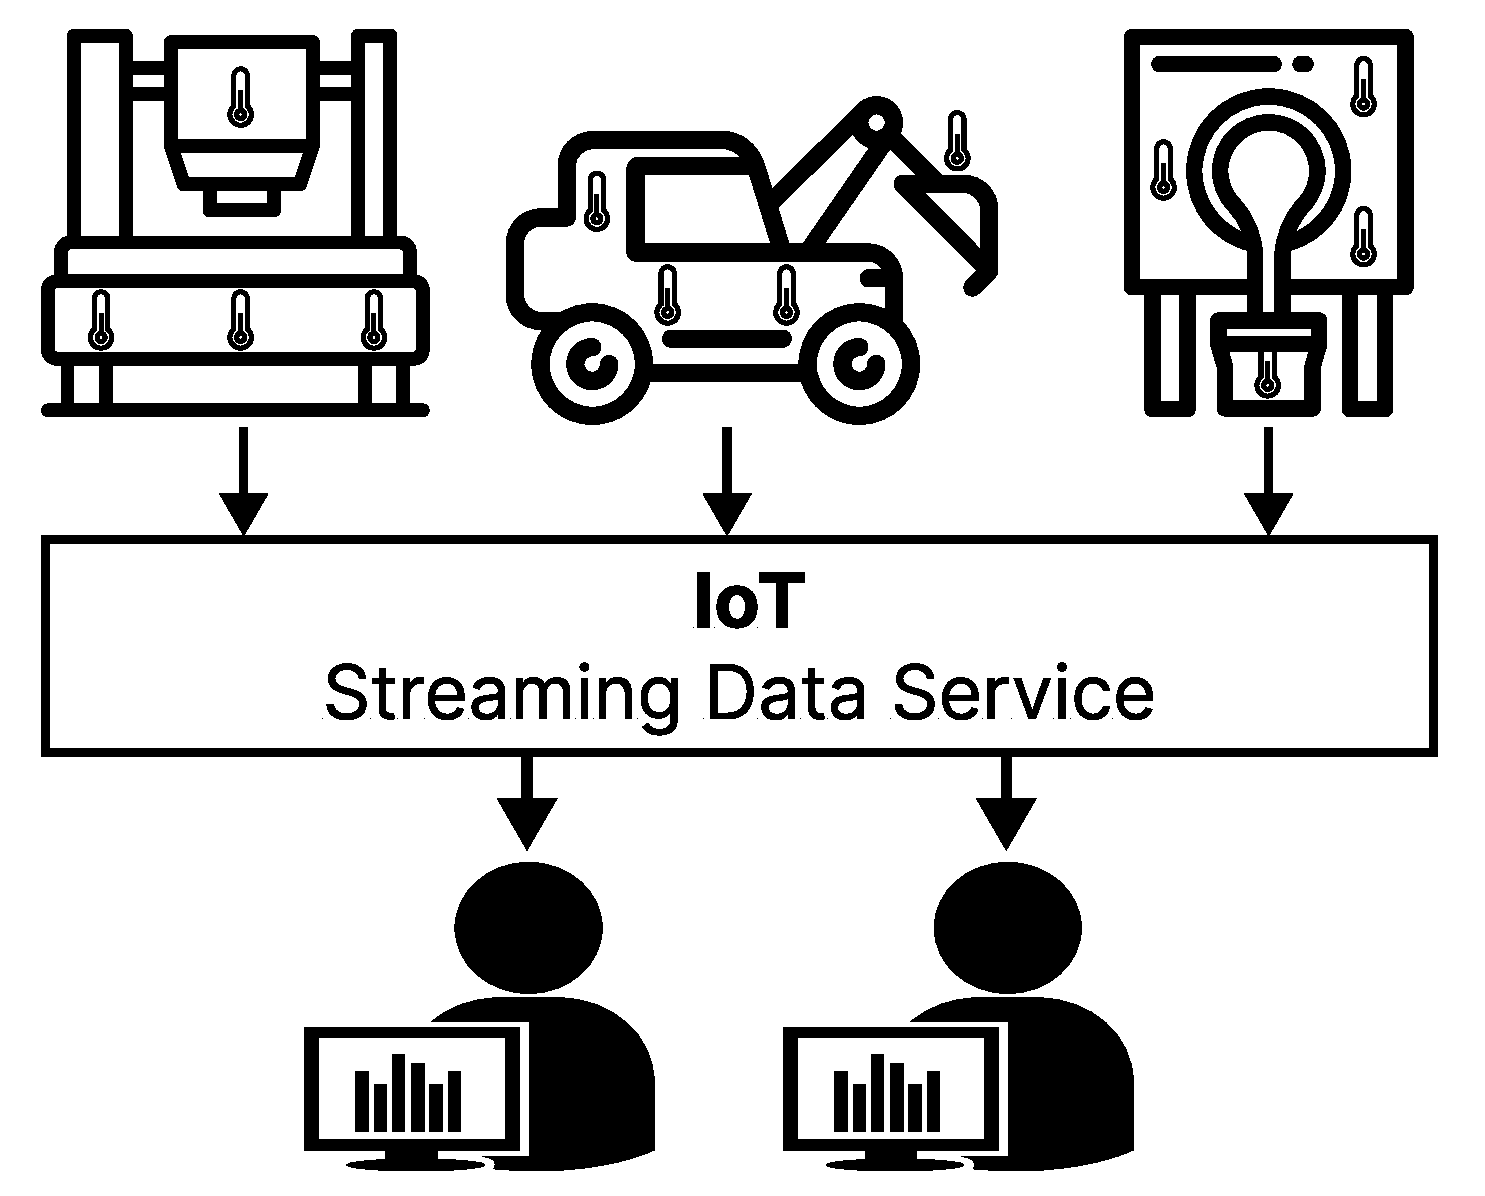
\includegraphics[width=\linewidth]{iot_example_schematic.pdf}
\caption{Schematic of the IoT streaming data service example}
\label{fig:iot_example}
\end{figure}

For example, consider a simple IoT streaming data service that monitors temperature sensors on large pieces of machinery as visualized in Figure~\ref{fig:iot_example}. Each machine is equipped with dozens of sensors that collect a temperature reading every second. Users monitor the machines by querying for temperature aggregates at different levels of granularity.

The input data for our data service consists of sensor information and sensor readings. The data maps onto the following table structure\footnote{We are using a pseudo-SQL syntax for the examples in this paper and assume basic familiarity with SQL. We recommend~\cite{} as an introduction to SQL.}:
\begin{lstlisting}[language=SQL]
CREATE TABLE Sensors (
    sensorid int,
    machineid int
);

CREATE TABLE SensorReading (
    sensorid int,
    time timestamp,
    temperature decimal
);
\end{lstlisting}

To get a broad overview, users look at one hour temperature averages over the last week, month, or other recent time period. To analyze a machine's recent performance they observe one minute averages over the last hour. In both cases, we use the median temperature over the last minute for each sensor to smooth the data and remove outliers.

We can express these data transformations and aggregates as a set of 3 views over the input data\footnote{In the view definitions, \emph{avg} and \emph{max} are aggregate functions whereas \emph{minute} and \emph{hours} are time windowing functions that round a timestamp to the next minute and hour, respectively.}:

\begin{lstlisting}[language=SQL]
CREATE VIEW SensorSmoothReading AS
SELECT sensorid,
    minute(time) as time_min,
    median(temperature) as temp
FROM SensorReading
GROUP BY sensorid, time_min
\end{lstlisting}

\begin{lstlisting}[language=SQL]
CREATE VIEW MachineHourReading AS
SELECT machineid,
    hour(time_min) as time_hour
    avg(temp) as avg_temp
    max(temp) as max_temp
FROM Sensors s
    JOIN SensorSmoothReading r
    ON r.sensorid = s.sensorid
GROUP BY machineid, time_hour
\end{lstlisting}

\begin{lstlisting}[language=SQL]
CREATE VIEW MachineMinuteReading AS
SELECT machineid, time_min
    avg(temp) as avg_temp
    max(temp) as max_temp
FROM Sensors s
    JOIN SensorSmoothReading r
    ON r.sensorid = s.sensorid
GROUP BY machineid, time_min
WHERE time_min + 1 HOUR >= now()
\end{lstlisting}

\emph{"View"} is a database term \ref{} for a table that is defined as a query over other tables and views. A view is a derived table that transforms table data into useful result sets by joining, aggregating, and analyzing rows from existing tables. Those may be intermediate result sets, like the \emph{SensorSmoothReading} view or views that are ultimately queried by end users and applications like the \emph{MachineHourReading} and \emph{MachineMinuteReading} views.

The IoT streaming data service exposes two API endpoints that query the respective views
\begin{lstlisting}[language=SQL]
MachineHourReading(machineid: Int!,
                   after: DateTime)
MachineMinuteReading(machineid: Int!)
\end{lstlisting}
The application calls those endpoints to fetch monitoring data for users.

In general, a streaming data service can be defined by a set of complex views over external sources of data\footnote{Some of the sources may be static or infrequently changing data. However, to be considered a \emph{streaming} data service, at least one source of data must be a data stream or update frequently (i.e. have a change stream)} and an API that queries those views.

In Section~\ref{sec:viewstore} we show that existing database technologies cannot efficiently implement such queried view sets with low latency and high throughput. We propose \emph{View Store} as a category of database systems that determine and execute optimal partial view materialization to support streaming data service use cases with low latency, high throughput querying on predefined views. Section \ref{sec:datasqrl} outlines the implementation of a view store called \emph{DataSQRL} and introduces the unique challenges of view store implementations.

SQL lacks some features needed to implement streaming data services. For our IoT example, we want to implement automatic alerts when machine temperatures exceed a certain threshold. SQL does not support "reacting" to changes in data and does not support data streams natively. We propose an extension of SQL called \emph{SQRL} - for \emph{Structured Query and \textbf{Reaction} language} - in Section \ref{sec:sqrl} that distinguishes between streaming and stateful data and adds the concept of \emph{subscriptions} for reacting to changes in data. SQRL adds some additional convenience features like incremental view definitions and explicit relationships to SQL that improve developer productivity when implementing streaming data services without changing the semantics of the relational algebra that SQL is based on.

We conclude this paper with a review of common streaming data service use cases, their implementation in SQRL, and compare the performance of DataSQRL to popular relational database systems like Postgres, MySQL as well as special-purpose databases like Neo4j and Timescale in Section \ref{sec:experiments}. Our experiments show that DataSQRL outperforms existing database engines by a factor of x-y. More significant, but also harder to measure, are the improvements in productivity that developers gain by using DataSQRL for their streaming data service implementations.

\section{Implementing Streaming Data Services}
\label{sec:viewstore}

In this section we review current approaches to implementing streaming data services using our IoT example and demonstrate the need for a new type of database system, called \emph{View store}, that support partial maintenance of complex views over streams of data.

A straight-forward way to implement the IoT example would be to write the sensor readings into a database table, install the views defined above, and execute the application queries against those views. We are going to outline how such implementations would perform in practice on various types of database systems.

\subsection{Transactional Database}

A transactional (i.e. row-oriented) database like Postgres \ref{}, MySQL \ref{}, SQLServer \ref{}, or Oracle \ref{} would be able to quickly ingest the streaming sensor data. However, executing the first query asking for a week of average machine temperatures would require retrieving and aggregating over 6 million records for a machine with 10 sensors. Even with carefully tuned index structures and compaction strategies, the data would likely be scattered over multiple non-consecutive disk pages which leads to lengthy data fetch operations that exceed our latency requirements. To reliably achieve responsive query answers within 100 milliseconds\footnote{100 milliseconds is widely considered the threshold for responsive user interactions.} the data would need to be held in memory. However, that is very expensive for the amount of data we are dealing with. Assuming we are monitoring 10000 machines with an average of 20 sensors each, we ingest half a trillion records a month. And even with powerful hardware that has this much RAM, the tail query latencies for machines with 100s of sensors would likely still exceed the 100 millisecond latency threshold when the workload is high (i.e. many users are concurrently monitoring machines).

\subsection{Data Warehouse}

A data warehouse (i.e. column-oriented) database like BigQuery \ref{}, Snowflake \ref{}, Redshift \ref{}, or Vertica \ref{} would reduce the cost of storing the data because of greater storage efficiency, usage of cheaper secondary storage modes, and absence of index structures. However, a data warehouse would not be able to achieve low latency response times to our queries. A data warehouse is optimized for queries that scan a large percentage of the entire stored data. While 6 million records is a substantial amount of data, it is a tiny fraction of the total data stored which makes column scans inefficient. Assuming we are monitoring 10000 machines, our queries would filter out all but 0.01\% of data. Even on powerful hardware, a data warehouse would be unable to achieve low latency response times when the workload is high because of the cost of those expensive scans.

\subsection{Analytics Engine}

The downside to using either type of database system is that we are storing a lot of data that the user isn't directly querying for which is costly in terms of data storage and the computation needed at query time. An analytics engine like Apache Spark \ref{} or Hadoop \ref{} is able to precompute the \emph{MachineHourReading} and \emph{MachineMinuteReading} views in batch and store only the resulting rows in a database for query answering. That greatly reduces the amount of data stored in the database and the computation needed to return the user query results. However, the downside of using an analytics engine in combination with a database is the long latency until new sensor readings can be queried. If we re-compute the views every hour, we have to wait up to 60 minutes before sensor readings can be queried. That's not acceptable since users may not be able to spot issues with the temperature before it is too late. Recomputing views very often is expensive since we have to read the entire data and compute all the aggregates before writing them into the database. And even if we use a lot of hardware, it will likely still takes minutes for the entire batch computation process and database update to complete.

\subsection{State of the Art}

Using existing data systems to implement streaming data service is either too expensive or does not meet latency requirements. Our simple IoT use case demonstrates that (in-memory) databases are too expensive for the data volume and have high tail query latencies, data warehouses do not meet our query latency requirements, and analytics engines do not meet our data latency requirements.

To implement streaming data services in practice, developers have to build custom architectures that combine multiple data systems to achieve the latency requirements at reasonable cost.

A popular approach is the lambda architecture \ref{} which combines the periodic batch computation of the analytics engine with a feed that writes recent data directly into the database. At query time, the data from the batch computed view is combined with the recent data to provide an up-to-date view.

Another approach is to build a data pipeline with custom scripts that build incrementally maintained materialized views which are stored in a database for querying.

Custom architectures are complex, expensive to implement and maintain, and hard to reason about. For every streaming data service use case, developers have to build a custom, hand-tuned database engine from multiple components that need to be orchestrated. Building such architectures that work reliably in practice, accommodate edge cases, and can be holistically monitored requires an extraordinary amount of work and expertise.

The high cost and lack of developer expertise result in implementation failures and lack of adoption of streaming data services despite the benefits they provide to data-driven applications.

\subsection{View Store}
\label{sec:viewstoredef}

We propose \emph{View Store} as a type of database system that meets the requirements of streaming data services and fills the gap in the current database landscape.

A view store is a database system that supports low latency, high throughput querying on a set of pre-defined views over multiple external sources of streaming data.

Let's look at the 3 elements that define a view store in more detail.

To meet the requirements of streaming data services, a view store has to provide low query and data latencies with high query and data throughput.
The time it takes to process new data is called the \emph{data latency} which measures the time from new data being available until all updates triggered by that data have been processed and the results are accessible. The time it takes to answer an application request is called the \emph{query latency} which measures the time that it takes to answer a request for data and return the result. Data latency requirements for streaming data services are usually on the order of seconds whereas query latency requirements are on the order of 100 milliseconds\footnote{Required latency times differ between use cases. The numbers provided here are best practice requirements across a number of use cases}.
The number of new data records that need to be ingested and processed across all data sources per time interval is called the \emph{data throughput}. The number of user or application requests that must be answered per time interval is called the \emph{query throughput}.

A view store requires that the set of views and the API which queries those views are defined prior to usage so that they can be compiled and optimized for efficient querying. That's the biggest difference to traditional database systems which allow arbitrary queries and optimize query execution at runtime\footnote{Most databases treat views as registered queries and allow for arbitrary queries at runtime}. However, the API of streaming data services only changes with the deployment cycle of the application and updates infrequently. And when it changes, those changes go through a deployment process. View stores take advantage of the fact that the views and queries are known in advance by investing resources up front in optimizing the data ingestion pipeline to reduce latencies at query time. Knowing the views, structure of the queries, and sources of data over which those are defined allows a view store to determine the optimal materialization strategy. Whereas traditional database systems find the fastest query plans against pre-defined data and index structures, a view store determines the optimal tradeoff between (partial) view materialization and query plans against the materialized views to meet latency requirements at low cost. We discuss optimization in more detail in Section~\ref{sec:optimization}.

Lastly, view stores consume data from one or multiple sources of streaming and static data. Most database systems assume that the data is explicitly inserted into pre-defined data structures. Federated database systems support multiple sources of data but do not support low query latencies for complex views since they need to fetch the data from the source systems at query time. View stores consume external data but build their own internal data structures to provide fast query access.

View stores are a specialized type of database system that meet the requirements of streaming data services. As streaming data services become more prevalent, we need view stores as a dedicated database category to support their implementation.
In Section~\ref{sec:datasqrl} we outline the implementation of the DataSQRL view store and provide more details on how view stores differ from other types of databases.

\section{SQRL}
\label{sec:sqrl}

SQRL, which stands for "Structured Query and Reaction Language", is an extension to the database query language SQL that accommodates the following needs of streaming data service implementations: 1) natively supporting streams of data and being able to "react" to changes in data, 2) increasing developer productivity for defining sets of complex views, 3) explicitly defining relationships and local scopes, 4) natively handling hierarchical data, and 5) providing flexible, programmatic query access via API.

The motivation for SQRL is twofold. First, SQRL adds features to SQL needed for handling streaming data - in particular, converting between streams and state to \emph{react} to changes in data and hence the "R" in "SQRL".
Second, SQRL adds a number of developer productivity and convenience features to make the language more appealing to software developers of streaming data services.

SQRL does not change the semantics of SQL and is based on the same relational algebra. SQRL is transpiled to SQL as described in Appendix~\ref{appendix:sqrl2sql}, but the resulting syntax tends to be much more verbose, harder to understand, and less efficient.

\subsection{Reacting to Data Changes: State vs Events}

A streaming data service often needs to react to changes in the data.
For our IoT example, we want to be alerted when the maximum temperature on a machine exceeds $100^{\circ}$ Celsius and define the view $HighTemp$ to capture such instances.

\begin{lstlisting}[language=SQL]
CREATE VIEW HighTemp AS
SELECT machineid, time_min, max_temp
FROM MachineMinuteReading
WHERE max_temp > 100
\end{lstlisting}

The $HighTemp$ view is based on the $MachineMinuteReading$ view that aggregates sensor readings by machine, which in turn is based on the $SensorSmoothReading$ view that aggregates sensor readings from the $SensorReading$ table into one minute buckets. In a streaming data service, sensor readings are appended to the $SensorReading$ table every second that a sensor produces a temperature reading and we want those readings to percolate through all the intermediate views up to the $HighTemp$ view to alert us to high temperatures. In other words, $SensorReading$ is a streaming table and the sequence of views defined on top of it form a data stream.

SQRL distinguishes between \emph{stream} and \emph{state} tables and views to support reacting to streams of data as well as handling relational data that represents state. Both stream and state tables/views\footnote{We use "table" and "view" interchangeably to describe the relations defined with SQRL. We use "table" for relational data that is imported and "view" for relations that are defined as queries against other relations}  are relations. \emph{Relation} is a database term for data records represented as rows with column structure. However, SQRL treats stream and state views differently for efficiency reasons.

A stream table is an append-only set of records that represent events in time. Every record in a stream table has a timestamp of the time when the event represented by the record took place. We use $timestamp(t)$ to denote the timestamp column of table $t$. $SensorReading$ is a stream table with $time$ as the timestamp column, i.e. $timestamp(SensorReading) = time$.

SQRL assumes that all events occur on a single, monotonically increasing timeline and that events arrive in order, i.e. that the timestamps are monotonically increasing. This is a simplifying assumption that is not true for real world systems. Section~\ref{sec:datasqrl-source} discusses how that assumption is relaxed in the DataSQRL system implementation without changing the semantics of SQRL.

A state table is a set of records that represents the state of entities. Rows in state tables can change over time as the state of the represented entity changes. For example, the $MachineSensorCount$ view is a state view which keeps track of how many sensors have been placed on each machine.

\begin{lstlisting}[language=SQL]
CREATE VIEW MachineSensorCount AS
SELECT machineid,
       count(*) as sensorcount
FROM Sensors
GROUP BY machineid
\end{lstlisting}

If we place another sensor on the machine with id $1075$, the row with $machineid = 1075$ will increment the value of $sensorcount$ by 1.

State tables have a natural key (i.e. a subset of columns) which uniquely identify the entity of which a particular row in the table represents its state. For $MachineSensorCount$ the natural key is $machineid$ which uniquely identifies the machine for each sensor count row in the view. We expect there to only be a single row for each $sensorid$ since a sensor can only be placed on one machine at a time. In contrast, we make no such uniqueness assumptions for streaming data.

SQRL treats all input tables as stream tables by default and supports converting stream to state tables. That means, the $Sensors$ input table is a stream table. If the input data guarantees that there is only one record for each $sensorid$ there is no significant semantic difference between a stream and state table.
However, if we want to allow moving sensors between machines, the $Sensors$ table contains the change-stream of sensor placements over time. That means, it can contain multiple records with the same $sensorid$ and different $machineid$. This changes the semantics of the $MachineSensorCount$ aggregate view because each sensor would count toward \emph{all} the machines it was ever placed on.
Instead, we want to capture the state of each sensor and only count it toward the machine it is currently placed on.

SQRL provides the \emph{DISTINCT ON} statement to convert streams to state based on a natural key:
\begin{lstlisting}[language=SQL]
CREATE VIEW Sensors AS
DISTINCT Sensors ON sensorid
    ORDER BY _source_time DESC;
\end{lstlisting}
This definition redefines the \emph{Sensors} table as a state view by taking the most recent change record for each \emph{sensorid} as the current state. This statement guarantees that there is only a single row per sensor id which contains the latest state or that sensor.
The \emph{\_source\_time} column is automatically added to all input table rows and captures the time that the source system from which the record was ingested attached to the record (e.g. the timestamp of a message in a queue). For streaming data sources that don't have an explicit timestamp column the \_source\_time column provides a useful alternative. Section~\ref{sec:datasqrl-source} discusses timestamp definition and inference in more detail.

The \emph{DISTINCT ON} statement converts a data stream of changes into a state view by taking the first row according to the specified order for each unique value of the natural key columns specified after \emph{ON}.

By redefining the $Sensors$ table as a state table before the $MachineSensorCount$ view is defined, we ensure that the latter only counts the current sensor placement states.

We can also use the familiar \emph{SELECT DISTINCT} statement to convert stream to state tables by deduplicating a data stream into unique data tuples. For example, we define a state view that contains all the machines we are monitoring as follows:
\begin{lstlisting}[language=SQL]
CREATE VIEW Machines AS
SELECT DISTINCT machineid
FROM Sensors
\end{lstlisting}

Similarly, \emph{GROUP BY} statements on stream tables produces state tables if the grouping key does not contain the timestamp column or timestamp function. The original $MachineSensorCount$ view is an example of creating a state aggregate over a stream.

A \emph{GROUP BY} statement on a stream table with a timetamp column or function in the grouping produces a stream view that contains a record for each group once the time window of the group is \emph{closed}. A time window is closed when the timeline has advanced far enough that any future stream records must have a timestamp that is larger than the upper end of the time window.

$SensorSmoothReading$ is an example of stream view created by a \emph{GROUP BY} on the underlying $SensorReading$ stream table because $time\_min$ is a timestamp function. A timestamp function is of the form $time\_func(timestamp)$ where $timestamp$ is the timestamp of the stream table and $time\_func$ is a monotonic function. In the case of $SensorSmoothReading$ the timestamp column is $time$ and the function is $minute$ which rounds the timestamp to the next minute and is therefore monotonic. $minute(time)$ creates time windows that are one minute wide.

Suppose we are currently aggregating for the group $(sensorid = 101, time\_min = 2022-05-01 15:08)$ which means that we take the median of all temperature readings from $SensorReading$ where $sensorid = 101$ and the time falls into the time window from $15:07:01$ to $15:08:00$ on May 1st. As soon as the timeline advances to $15:08:01$ the time window for the group is closed and creates record with the median temperature computed up to this point. The monotonicity of the timeline guarantees that we won't encounter any older stream records that would need to be added to this time window.

In other words, \emph{GROUP BY} stream views have an implied \emph{HAVING} clause that filters out groups where the upper end of the time window is bigger or equal to the current time on the timeline. Formally, the condition is $time\_func(timestamp) < time\_func(now())$ where $now()$ is the current time of the timeline.
SQRL provides the special \emph{now()} function which stands for the current time as a convenient way to define sliding time windows and filter records by recency. The $MachineMinuteReading$ view is an example that uses $now()$ to restrict records to a recent time window by filtering in the \emph{WHERE} clause. $now()$ is another means for converting a stream to state by defining a "recent state". The specifics of $now()$ are discussed in more detail in Appendix~\ref{appendix:sqrl2sql}.

The timestamp of a stream created by \emph{GROUP BY} is the timestamp column or function used in the grouping. The timestamp column of the $SensorSmoothReading$ is $time_min$.

SQRL converts stream tables and views to state views when using \emph{DISTINCT ON}, \emph{SELECT DISTINCT}, \emph{GROUP BY} without time window, and filtering with $now()$. To convert from state to stream, SQRL provides the \emph{SUBSCRIBE TO} construct.

For example, we want to alert the monitoring staff when a machine has more than 1000 sensors because such massive machines require special attention.

\begin{lstlisting}[language=SQL]
BigMachines := SUBSCRIBE ON ADD TO
SELECT machineid, sensorcount
FROM MachineSensorCount
WHERE sensorcount >= 1000
\end{lstlisting}

This example defines the \emph{BigMachine} stream view as a subscription which creates an event record with \emph{machineid} and \emph{sensorcount} whenever a machine in the \emph{MachineSensorCount} view has more than 1000 sensors. We call the view definition of a subscription (i.e. the part after "TO") the \emph{observed view}.

A subscription specifies which type of change against the observed view creates an event:
\begin{enumerate}
    \item \textbf{ON ADD}: Creates an event record whenever a row is newly added to the observed view.
    \item \textbf{ON CHANGE}: Creates an event record whenever a row in the observed view changes
    \item \textbf{ON DELETE}: Creates an event records whenever a row is removed from the observed view.
\end{enumerate}

Observed views of subscriptions are state views from which events are created upon certain observed changes. Those events are the stream view defined by the subscription. A subscription stream view has an $\_event\_time$ column with the timestamp of the triggering event that can also be accessed via the special function $event\_time()$.

Filters (\emph{WHERE}) and projections (\emph{SELECT}) do not affect the type of a table of view. However, join operators require special consideration.

Joining two tables of the same type has the join semantics of standard relational algebra and produces a relation of the same type. When joining two stream tables $A$ and $B$, the $\_event\_time$ timestamp column contains the maximum timestamp of the two joined records unless the join has the condition $timestamp(A) >= timestamp(B)$ in which case the timestamp of table $A$ is the timestamp of the joined record.

When joining a stream with a state table, the result is a state table under the standard join semantics. However, in most use cases the intended result is a stream of records that joins the stream event against the state at the time of the event.

For example, to track the highest temperature reading per machine over the last 24 hours, we might define the following view:
\begin{lstlisting}[language=SQL]
CREATE VIEW MachineRecentMaxTemp AS
SELECT machineid,
    max(temp) as max_temp
FROM Sensors s
    JOIN SensorSmoothReading r
    ON r.sensorid = s.sensorid
WHERE time_min + 24 HOUR >= now()
GROUP BY machineid
\end{lstlisting}

However, if the join in this example is interpreted as an inner join between state view $Sensors$ and the stream view $SensorSmoothReading$ then moving a sensor $s$ from machine $m1$ to $m2$ would result in the last 24 hours of sensor readings from $s$ to be reassigned from $m1$ to $m2$. Hence, $MachineRecentMaxTemp$ would be a state view that changes over time with sensor placement. However, the intended result is for sensor readings to be assigned to the machines that the sensor was placed on at the time of the reading. Since this is a very common use case for joining state with stream data in streaming data services, SQRL introduces the \emph{TEMPORAL JOIN}.

A \emph{TEMPORAL JOIN} is only defined between a stream and a state table and expands the join condition by the constraint that the records from the state table that participate in the join must have been valid at the time of the event from the stream table per the stream table's timestamp. A formal definition of temporal joins is provided in Appendix~\ref{appendix:sqrl2sql}. A temporal join preserves the timestamp of the stream table.

By default, a \emph{JOIN} between a stream and state is interpreted as a temporal join.

When building streaming data services it is important to distinguish between streaming and stateful data. SQRL extends SQL by features that make it easy to seamlessly convert between the two and combine data from different types.

\subsection{Developer Productivity}

SQL is a great language for defining queries over tabular data. For software development, developers prefer languages that are easy to read for larger bodies of code, convenient to use, and allow for incremental development. SQRL adds languages features to SQL to make it more developer friendly.

Developers implement streaming data services in SQRL scripts. An SQRL script first declares the (streaming) data sources that it builds on using \emph{IMPORT} statements. Our IoT example has the following imports:
\begin{lstlisting}[language=SQL]
IMPORT sensordata.SensorReading;
IMPORT sensordata.Sensors;
\end{lstlisting}

An import statement has two parts: the name of the data source and the name of the table to import from that source. Data sources can be queues, file systems, logs, etc and are configured under a unique name. We discuss data sources in more detail in Section~\ref{sec:datasqrl-source}.
We can also import all tables from a data source via \emph{IMPORT sensordata.*}. Once imported, the tables can be referenced in \emph{FROM} clauses of view definitions.

To reduce the verbosity of the SQL view definition syntax, SQRL adds the assignment operator $:=$ as a syntactic shorthand for definitions.

\begin{lstlisting}[language=SQL]
SensorSmoothReading := SELECT sensorid,
    minute(time) as time_min,
    median(temperature) as temp
FROM SensorReading
GROUP BY sensorid, time_min
\end{lstlisting}

SQRL automatically infers whether a view is a stream or state based on the definition. The developer can also explicitly declare the type in front of a definition to make the type explicit. Such type declaration is optional and does not change the semantics of the script. However, the compiler will return an error if the declared type does not match the inferred.

\begin{lstlisting}[language=SQL]
STREAM SensorSmoothReading :=
SELECT sensorid,
    minute(time) as time_min,
    median(temperature) as temp
FROM SensorReading
GROUP BY sensorid, time_min
\end{lstlisting}

SQRL supports incremental view definitions and redefining existing views and columns. This is particularly useful for data cleansing and data normalization which are frequently part of streaming data service implementations.

For example, most of our sensors produces readings with a \emph{temperature} column that contains the Celsius value. However, some older sensors produce a reading with a \emph{temperature\_f} column in Fahrenheit. To normalize the data, we redefine the \emph{temperature} column on the \emph{SensorReading} table as follows.

\begin{lstlisting}[language=SQL]
SensorReading.temperature :=
    coalesce(temperature,
        (temperature_f - 32)/9*5)
\end{lstlisting}

This statement overrides the \emph{temperature} column so that any subsequent references to that column table resolve to the correct temperature.

SQRL scripts can import views defined by other scripts in order to facilitate reuse of data transformations and analytics between data services. To share our definition of \emph{SensorSmoothReading} between scripts, we can place it in a script called \emph{sensorshared} and then import the view:
\begin{lstlisting}[language=SQL]
IMPORT sensorshared.SensorSmoothReading
\end{lstlisting}

All public views and columns are accessible by the importing script. Views and columns with names starting with an underscore are private and not accessible outside the script.

To connect stream views to outside consumers, SQRL provides \emph{EXPORT} statements.
\begin{lstlisting}[language=SQL]
EXPORT HighTemp TO alerts.TempAlert
\end{lstlisting}
Assuming we have a data sink with the name \emph{alerts} registered, this statement exports all event records from the $HighTemp$ stream into the data sink under the \emph{TempAlert} namespace. If the exported table/view is of type state, then the change stream is exported. In other words, $EXPORT\ State\ TO\ x$ is implicitly converted to:
\begin{lstlisting}[language=SQL]
EXPORT
  (SUBSCRIBE ON CHANGE TO State)
TO x
\end{lstlisting}

\subsection{Relationships and Local Scopes}

SQRL adds the concept of \emph{relationships} to SQL in order to improve code readability, simplify the conceptual model, and make it easier to handle hierarchical data.

A column can be defined as a relationship column using a JOIN clause to relate rows from one table or view to those from another.
\begin{lstlisting}[language=SQL]
Sensors.readings :=
JOIN SensorSmoothReading r
    ON r.sensorid = @.sensorid
\end{lstlisting}

This statement defines a relationship column \emph{readings} on the table \emph{Sensors} as a natural join with \emph{SensorSmoothReading}.
The underscore in the join condition is the alias for the view on the left-hand side of the assignment operator, i.e. \emph{Sensors}, that's automatically assigned by SQRL.

Relationship columns represent a logical join that gets instantiated when the column is accessed in a view definition or column expression. For example, we can simplify the join clause of the \emph{MachineRecentMaxTemp} view using the relationship column:
\begin{lstlisting}[language=SQL]
CREATE VIEW MachineRecentMaxTemp AS
SELECT machineid,
    max(temp) as max_temp
FROM Sensors s JOIN s.readings r
WHERE time_min + 24 HOUR >= now()
GROUP BY machineid
\end{lstlisting}

The join with \emph{s.readings} expands to the full join declaration from above with the table alias $s$ filling in for the underscore alias placeholder, which means the above view definition is equivalent to the original one.

Relationship columns allow us to reuse join declarations across view definitions and column expressions as well as label a relationship explicitly to support code readability.

Another feature that SQRL introduces is the concept of localized scopes to break out sub-queries and define them incrementally. For example, if we wanted to add $sensorcount$ as a column on the $Machines$ view instead of tracking it in a separate view, we could update the \emph{Machines} view as follows:

\begin{lstlisting}[language=SQL]
CREATE VIEW Machines AS
SELECT machineid,
(SELECT count(*) FROM
Sensors s WHERE
s.machineid = m.machineid)
    AS sensorcount
FROM
(SELECT DISTINCT machineid
FROM Sensors) m
\end{lstlisting}

View definitions with nested sub-queries are hard to read. In SQRL we can break out the $sensorcount$ sub-query and implement it as an incremental column definition:
\begin{lstlisting}[language=SQL]
Machines.sensorcount :=
SELECT count(*) FROM
Sensors s WHERE
s.machineid = @.machineid
\end{lstlisting}

This statement adds the $sensorcount$ column to the previously defined $Machines$ view. The underscore refers to the $Machines$ view on the left-hand side of the assignment and defines this query in localized scope, i.e. as a nested sub-query.

Localized scope is particularly useful in combination with relationships. Instead of defining the entirely separate view \emph{MachineRecentMaxTemp} to capture the maximum recent temperature of a machine, we can do so by adding another relationship and column to \emph{Machines}:

\begin{lstlisting}[language=SQL]
Machines.sensors := JOIN Sensors s
    ON s.machineid = @.machineid

Machines.maxTemp :=
SELECT max(temp) FROM @.sensors.readings
WHERE time_min + 24 HOUR >= now()
\end{lstlisting}

$sensors$ defines a relationship column that relates rows in $Machines$ to the $Sensors$ that are placed on them through a natural join. The $maxTemp$ column is a localized sub-query that aggregates the maximum temperature for all sensors readings per machine. The expression $\@.sensors.readings$ is a concatenated relationship expression that combines the join declarations from the two relationships.
The complete view definition in SQL is shown in Figure~\ref{fig:machinesView} and demonstrates the convenience and utility of SQRL sytnax.

\begin{figure*}
\begin{lstlisting}[language=SQL]
CREATE VIEW Machines AS SELECT machineid,
   (SELECT count(*) FROM Sensors s
    WHERE s.machineid = m.machineid) AS sensorcount
   (SELECT max(temp) FROM Sensors s
    JOIN SensorSmoothReading r ON r.sensorid = s.sensorid
    WHERE s.machineid = m.machineid AND
          time_min + 24 HOUR >= now()) AS maxTemp
FROM (SELECT DISTINCT machineid FROM Sensors) m
\end{lstlisting}
\caption{Example of how SQRL syntax expends to standard SQL}
\label{fig:machinesView}
\end{figure*}

To compute the current temperature of each machine as the average of the most recent temperature reading for all sensors on the machine, we define a $lastReading$ relationship on sensors that relates a sensors to it's most recent temperature reading:

\begin{lstlisting}[language=SQL]
Sensors.lastReading :=
JOIN SensorSmoothReading r
    ON r.sensorid = @.sensorid
    ORDER BY r.time_min DESC LIMIT 1
\end{lstlisting}

Adding a \emph{LIMIT} to the join clause of a relationship definition constrains the multiplicity of the relationship. The \emph{ORDER BY} clause determines which related records are part of the relationship. We use the $lastReading$ relationship to compute the temperature average as follows:

\begin{lstlisting}[language=SQL]
Machines.currentTemp := SELECT avg(temp)
    FROM @.sensors.lastReading
\end{lstlisting}

Expressing a multiplicity restricted join in SQL is cumbersome and requires a nested \emph{PARTITION OVER} query that assigns a row number to filter on. Figure~\ref{fig:machinesPartitionOver} shows the equivalent SQL syntax.

\begin{figure*}
\begin{lstlisting}[language=SQL]
CREATE VIEW Machines AS SELECT machineid,
   ...
   (SELECT avg(temp) FROM Sensors s JOIN
     (SELECT sensorid, temp FROM
        (SELECT sensorid, temp,
        row_number() OVER (PARTITION BY sensorid ORDER BY time_min DESC)
            AS row_no
        FROM SensorSmoothReading)
     WHERE row_no = 1) r ON r.sensorid = s.sensorid
   WHERE s.machineid = m.machineid) AS currentTemp
FROM (SELECT DISTINCT machineid FROM Sensors) m
\end{lstlisting}
\caption{Example of how SQRL syntax expends to standard SQL}
\label{fig:machinesPartitionOver}
\end{figure*}

When aggregating a single column over a to-many relationship, SQRL supports a convenience syntax to specify the relationship path inside the aggregate function. This allows us to simplify the $currentTemp$ column definition to:

\begin{lstlisting}[language=SQL]
Machines.currentTemp :=
  avg(sensors.lastReading.temp)
\end{lstlisting}

\subsection{Representing Hierarchical Data}

Many data services need to consume hierarchically structured data such as JSON documents. SQRL natively supports hierarchical data through nested tables with parent-child relationships to eliminate the cumbersome work of mapping between hierarchical and relational data.

For example, our IoT application allows users to define \emph{monitoring groups} to monitor groups of machines, such as a fleet of vehicles or all machines on a factory floor. Monitoring Groups are stored as JSON objects like the following:

\begin{lstlisting}
{
  groupid: 501,
  groupName: "Wenatchee Factory",
  machines: [
   {
     machineid: 1075,
     machineName: "Mill Saw"
   },
   {
     machineid: 1098,
     machineName: "Wood Grinder"
   }
  ]
}
\end{lstlisting}

In SQRL, this data can be imported like any other table and converted to a state table:
\begin{lstlisting}
IMPORT iotapp.MonitorGroup;

MonitorGroup := DISTINCT MonitorGroup
    ON groupid
    ORDER BY _source_time DESC;
\end{lstlisting}

Internally, SQRL creates two tables: \emph{MonitorGroup} with columns $groupid$, $groupName$, and a relationship column $machines$ that relates to the respective rows in the nested table \emph{MonitorGroup.machines} which has the columns $machineid$, $machineName$, and a relationship column $parent$ which relates it back to the parent table row.

The relationships between the parent and child tables is based on their shared primary key. SQRL assigns a primary key to each imported table and defined view. The input stream tables are automatically assigned a universally unique identifier in the $\_uid$ column that SQRL appends to each incoming record. The primary key of state tables is the natural key. That means the columns after \emph{ON} for $DISTINCT\ ON$ statements, the columns selected in a $SELECT DISTINCT$ statement, or the grouping keys of a $GROUP BY$ clause.

In our example, the primary key of $Sensors$ is $sensorid$ because $Sensors$ is defined by a $DISTINCT\ ON$ statement with $sensorid$ as the $ON$ columns. The primary key of $Machines$ is $machineid$ because $Machines$ is defined by a $SELECT\ DISTINCT$ statement with $machineid$ as the only selected column. And the primary key of $MachineSensorCount$ is $machineid$ because $machineid$ is the only key in the $GROUP BY$ clause of the view definition.

When two tables or views are joined, the resulting relation is assigned the combined primary key. Filters and projections do not affect the primary key. SQRL always maintains the primary key on a table or view even if it is projected out in which case it is stored in hidden columns. SQRL maintains the primary key to trace lineage of records, ensure every record is identifiable, and generate unique ids for the API as discussed in Section~\ref{sec:sqrl_api}. $UNION (ALL)$, $INTERSECT$, and $EXCEPT$ have special semantics and primary key propagation depending on the type of tables/views involved as specified in Appendix~\ref{appendix:sqrl2sql}.

In the case of hierarchical data, SQRL creates a hidden primary key for the nested table that combines the primary key of the parent table with the local primary key of the nested table, e.g. the index offset in the array for our example data.

SQRL maps nested data onto separate tables related by shared primary key and uses relationship columns to explicitly relate the tables in the logical model to allow the user to navigate the hierarchical structure.

For example, we can compute the number of machines in a monitoring group by counting the relationship column:
\begin{lstlisting}[language=SQL]
MonitorGroup.numMachines :=
                count(machines)
\end{lstlisting}

Nested tables can be treated and extended like any other table with the only difference that nested table names are paths. For example, we can add a relationship column that relates the machines in a monitoring group to the \emph{Machines} view:
\begin{lstlisting}[language=SQL]
MonitorGroup.machines.machine :=
  JOIN Machines m
  ON m.machineid = @.machineid
\end{lstlisting}

SQRL automatically defines nested tables in the data model when the input data is hierarchically structured. In addition, the user can define nested views explicitly to group by the parent table or view.

For example, the following nested view computes the temperature maximums and averages by 1 hour time window for all the machines in a monitoring group:
\begin{lstlisting}[language=SQL]
MonitorGroup.hourReading :=
SELECT hour(time_min) as time_hour,
       avg(temp) as avg_temp,
       max(temp) as max_temp
FROM @.machines.machine.sensors.readings
GROUP BY time_hour
ORDER BY time_hour DESC
\end{lstlisting}

Because this query defines a nested view under the \emph{MonitorGroup} table, the grouping by parent table primary key is implied which simplifies the syntax. That means, $MonitorGroup.hourReading$ has the primary key ($groupid$,$time\_hour$) because the primary key of the parent $MonitorGroup$ table is $groupid$ (since it is defined by a $DISTINCT ON$ statement above) and the local key is the $GROUP BY$ key $time\_hour$.

Relationship columns, localized query statements, and nested tables support an object-oriented thinking that many developers are familiar with and simplifies query statements. By making relationships in the data explicit, developers can directly translate their conceptual entity-relationship model into SQRL without intermediate translation.

All of these features extend the syntax of SQL but not the semantics of the underlying relational algebra. Appendix~\ref{appendix:sqrl2sql} details how SQRL translates to SQL.

\subsection{Programmatic Query Access via API}
\label{sec:sqrl_api}

Streaming data services are accessed programmatically through an API from an application or developer code. SQRL supports GraphQL and REST APIs. Specifically, SQRL maps API specifications in GraphQL schema (for GraphQL) or OpenAPI 3.0 (for REST) onto queries over the views defined in an SQRL script. This gives developers the flexibility to define custom APIs based on the naming convention of their SQRL script without having to specify and implement an explicit mapping.

The following outlines the mapping of GraphQL schema onto view queries. The mapping for OpenAPI is analogous and all the details are provided in Appendix~\ref{appendix:sqrl2graphql}.

GraphQL types are mapped onto public tables or views defined in the SQRL script with the same name. The field names for such types must match the column names and the field types must be compatible (but not necessarily identical) with the type of the column. For scalar columns, that means that the column data type must be convertible to the field data type and vice versa. For relationship columns, the field type must be a reference to the type that maps onto the related table or any interface that this type implements.
Root queries defined in the GraphQL schema query the view that the query return type maps to. Any arguments of the query are mapped onto equality conditions for the column that has the same name as the argument, unless the data type of the argument is a range predicate (i.e. a NumberComparison or TimeComparison) in which case it is interpreted as a range constraint. In addition, $limit$, $offset$, and $order$ arguments of the query are mapped onto query limits, offsets, and order-by clauses, respectively. Such arguments can also be added to relationship fields in type definitions to constrain the query for the related table.

For our example, we define the following GraphQL schema fragment:
\begin{lstlisting}
type MonitoringGroup {
   nodeid: ID!
   groupid: Int!
   groupName: String!
   machines: [MonitoringGroup_machines!]!
   hourReading(limit: Int):
      [MonitoringGroup_hourReading!]!
}

type MonitoringGroup_machines {
  machineId: Int!
  machineName: String!
}

type MonitoringGroup_hourReading {
  time_hour: DateTime!
  avg_temp: Float!
  max_temp: Float!
}

type Query {
  group(groupid: Int!): MonitoringGroup
}
\end{lstlisting}

This schema defines a type for the $MonitoringGroup$ view as well as types for the two nested tables $machines$ and $hourReading$ which maps their respective columns. Note, that the relationship field $machines$ on $MonitoringGroup$ does not have any arguments and will return all machines in the group. The $hourReading$ field, on the other hand, supports a $limit$ argument to constrain how many rows from the nested view to return. Similarly, the root query $group$ has a required $groupid$ argument by which it queries $MonitoringGroup$ view.

A field with an $ID$ data type returns a unique identifier for each record of the type by exposing the determined primary key of the mapped table. These identifiers can be used by the consumer to establish equivalence and retrieve records.

This schema fragment supports the following GraphQL query over the views defined in our example SQRL script:

\begin{lstlisting}
group(groupid : 501) {
    groupName
    machines {
        machineId
        machineName
    }
    hourReading (limit: 24) {
        time_hour
        avg_temp
        max_temp
    }
}
\end{lstlisting}

This GraphQL query translates to a $SELECT$ query on the $MonitoringGroup$ view where $groupid = 501$. It also returns all the machines in that group and the last 24 hours of aggregate sensor readings by traversing through relationship fields. Developers can customize the API specification to their requirements by introducing interfaces, restricting types, adding arguments, etc. A complete description of the GraphQL schema to SQRL mapping is provided in Appendix~\ref{appendix:sqrl2graphql}.

Note, how the entity-relationship model of SQRL maps directly onto the type-reference model of GraphQL. This gives developers flexibility in defining their APIs without having to write explicit mapping code, thereby significantly reducing the object-relational impedence mismatch~\cite{} that most ORM libraries and database abstraction layers introduce.

\subsection{Complete Example}

\begin{figure*}[!ht]
    \begin{minipage}[l]{1.0\columnwidth}
        \centering
        \begin{lstlisting}[language=SQL]
IMPORT sensordata.*;
IMPORT iotapp.MonitorGroup;

Sensors := DISTINCT Sensors ON sensorid
    ORDER BY _source_time DESC

SensorReading.temperature :=
    coalesce(temperature,
        (temperature_f - 32)/9*5);

Sensors.readings :=
    SELECT minute(time) as time_min,
        median(temperature) as temp
    FROM SensorReading r
    WHERE r.sensorid = @.sensorid
    GROUP BY time_min;

Sensors.lastReading :=
    JOIN @.readings r
    ORDER BY r.time_min DESC LIMIT 1;

Machines := SELECT DISTINCT machineid
    FROM Sensors;

Machines.sensors := JOIN Sensors s
    ON s.machineid = @.machineid;

Machines.currentTemp :=
    avg(sensors.lastReading.temp);

Machines.maxTemp :=
    SELECT max(temp)
    FROM @.sensors.readings
    WHERE time_min + 24 HOUR >= now();

Machines.hourReading :=
    SELECT hour(time_min) as time_hour
        avg(temp) as avg_temp
        max(temp) as max_temp
    FROM @.sensors.readings
    GROUP BY time_hour;
    \end{lstlisting}
    \end{minipage}
    \hfill{}
    \begin{minipage}[r][][b]{1.0\columnwidth}
    \centering
    \begin{lstlisting}[language=SQL]
Machines.minuteReading :=
    SELECT time_min
        avg(temp) as avg_temp
        max(temp) as max_temp
    FROM @.sensors.readings
    GROUP BY time_min
    WHERE time_min + 1 HOUR >= now();

HighTemp := SELECT parent.machineid,
       time_min, max_temp
FROM Machines.minuteReading
WHERE max_temp > 100;

EXPORT HighTemp TO alerts.TempAlert;

Machines.sensorcount := count(sensors);

BigMachines := SUBSCRIBE ON ADD TO
SELECT machineid, sensorcount
FROM Machines
WHERE sensorcount >= 1000;

EXPORT BigMachines TO alerts.BigMachine;

MonitorGroup := DISTINCT MonitorGroup
    ON groupid
    ORDER BY _source_time DESC;

MonitorGroup.numMachines :=
                count(machines);

MonitorGroup.machines.machine :=
  JOIN Machines m
  ON m.machineid = @.machineid

MonitorGroup.hourReading :=
SELECT time_hour,
       avg(avg_temp) as avg_temp,
       max(max_temp) as max_temp
FROM @.machines.machine.hourReading
GROUP BY time_hour
    \end{lstlisting}
    \end{minipage}
\caption{Complete SQRL script for the IoT streaming data service}
\label{fig:complete_example}
\end{figure*}

The complete SQRL script for our running example is shown in Figure~\ref{fig:complete_example} which combines the SQRL code snippets discussed above. In the complete example, the \emph{SmoothSensorReadings} view is replaced by the nested view $Sensors.readings$. We also express the hour and minute temperature aggregates as nested views on the $Machines$ view. That allows us to refer $Machines.hourReading$ by its implied relationship with $Machines$ in the definition of $MonitorGroup.hourReading$ to simplify the relationship path in the $FROM$ clause to:
\begin{lstlisting}[language=SQL]
@.machines.machine.hourReading
\end{lstlisting}

Note, how the syntax of SQRL allows us to express a moderately complex streaming data service in a few lines of readily readable code without changing the core structure of SQL query and view definitions. In addition, the introduction of relationships, local scoping, and nested tables give SQRL an entity-centric conceptual model that aligns with the object-oriented thinking most developers are familiar with.

\begin{figure*}[!ht]
    \begin{minipage}[l]{1.0\columnwidth}
        \centering
        \begin{lstlisting}
scalar DateTime

type TimeComparison {
   before: DateTime
   after: DateTime
}

type Machines {
   nodeid: ID!
   machineid: Int!
   maxTemp: Float
   sensorcount: Int
   hourReading(time_hour: TimeComparison,
      limit: Int): [Machines_hourReading!]!
   minuteReading(limit: Int):
      [Machines_minuteReading!]!
}

interface Reading {
  avg_temp: Float!
  max_temp: Float!
}

type Machines_hourReading
    implements Reading{
  time_hour: DateTime!
  avg_temp: Float!
  max_temp: Float!
}

type Machines_minuteReading
    implements Reading{
  time_min: DateTime!
  avg_temp: Float!
  max_temp: Float!
}
    \end{lstlisting}
    \end{minipage}
    \hfill{}
    \begin{minipage}[r][][b]{1.0\columnwidth}
    \centering
    \begin{lstlisting}
type Floatomparison {
   larger: float
   largerOrEq: float
}

type MonitoringGroup {
   nodeid: ID!
   groupid: Int!
   groupName: String!
   machines: [MonitoringGroup_machines!]!
   hourReading(limit: Int):
      [MonitoringGroup_hourReading!]!
}

type MonitoringGroup_machines {
  machineId: Int!
  machineName: String!
}

type MonitoringGroup_hourReading
    implements Reading{
  time_hour: DateTime!
  avg_temp: Float!
  max_temp: Float!
}

type Query {
  group(groupid: Int!): MonitoringGroup
  machine(machineid: Int!): Machines
  machinesBySensor(sensorcount: Int!):
                [Machines!]!
  findMachines(sensorcount: Int,
  maxTemp: FloatComparison): [Machines!]!
}
    \end{lstlisting}
    \end{minipage}
\caption{Complete GraphQL schema API for IoT example}
\label{fig:complete_api}
\end{figure*}

The complete GraphQL API schema definition for our IoT streaming data service is shown in Figure~\ref{fig:complete_api}. It extends the previous API snippet by the Machine type and the nested sensor reading aggregates.

Note, how the developer is free to customize the API to their needs by selecting the types and fields they need, providing data access paths through arguments, customizing the structure through interfaces, and defining query endpoints. For example, in addition to retrieving machines by their id, we added two additional query endpoints to the API: $machinesBySensor$ returns all machines that have a certain number of sensors and $findMachines$ finds machines that have a certain sensor count and recently exceeded the optionally provided temperature.

\section{DataSQRL}
\label{sec:datasqrl}

DataSQRL is a view store implementation based on SQRL. The high-level architecture of DataSQRL is shown in Figure~\ref{fig:datasqrl_architecture}. The DataSQRL orchestrator provides an API for developers to compile and deploy SQRL scripts, connect data sources and sinks, and monitor the whole system.

\begin{figure}[h]
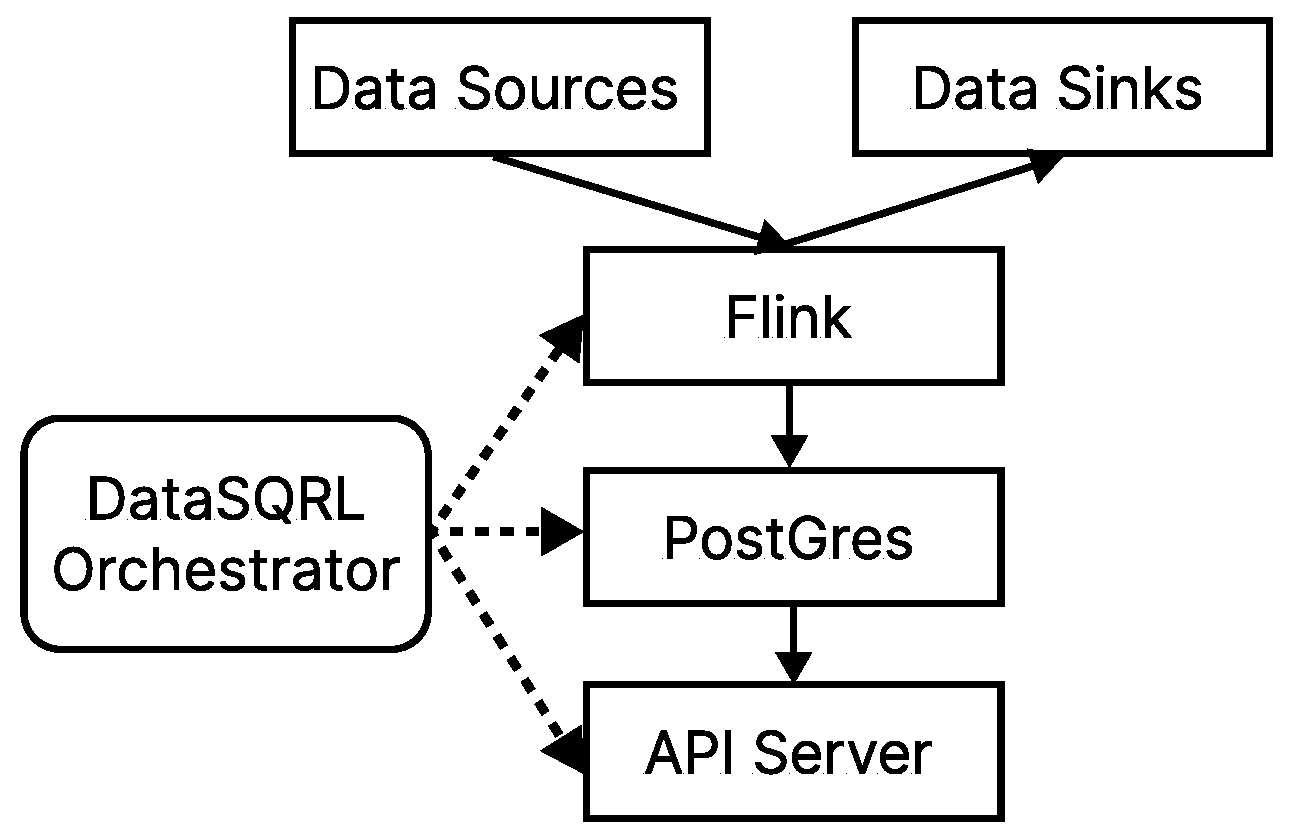
\includegraphics[width=\linewidth]{datasqrl_architecture.pdf}
\caption{High level architecture of DataSQRL}
\label{fig:datasqrl_architecture}
\end{figure}

DataSQRL uses Apache Flink~\cite{} for streaming data ingestion and view materialization. Flink consumes data from the connected data sources according to the data source configuration, processes the data, and writes the results into Postgres tables or publishes them to connected data sinks (for \emph{EXPORT} statements). The JobGraph that specifies the Flink stream execution is generated by the DataSQRL orchestrator. The orchestrator also generates views over the Postgres tables and installs them in the database. The DataSQRL API Server executes SQL queries against those views to respond to GraphQL and REST queries against the generated API based on the mapping defined by the API specification.

The combination of stream engine, database, and API server is a common architecture for streaming data services. What makes DataSQRL unique is that it generates all the data models, mappings, and data transformations needed to combine these systems efficiently from the SQRL script and API schema. Section~\ref{sec:compilation} describes how DataSQRL compiles SQRL scripts. DataSQRL determines what should be materialized by the stream engine as data is ingested versus what data should be computed at query time in the database. This tradeoff has a huge impact on the performance and cost of the system. Section~\ref{sec:optimization} discusses this tradeoff in more detail and describes the DataSQRL optimizer which automatically optimizes the tradeoff.

\subsection{Sources and Timestamps}
\label{sec:datasqrl-source}

The user configures data sources and sinks with DataSQRL, so that the system knows how to connect to the data contained therein and produce a suitable data source adapter for Flink.

All imported tables are stream tables. The developer can define the timestamp for a stream table in the import statement explicitly through the \emph{TIMESTAMP} keyword:
\begin{lstlisting}[language=SQL]
IMPORT sensordata.SensorReading
       TIMESTAMP time;
\end{lstlisting}

This import statement makes it explicit that the timestamp for the $SensorReading$ stream is the $time$ column. Timestamps can also be defined as expressions (e.g. to convert a column value to a $DateTime$ type) in which case the expression can be assigned to a new column on the table with the statement:

\begin{lstlisting}[language=SQL]
$IMPORT table TIMESTAMP
    expression AS column_name$.
\end{lstlisting}

If a timestamp is not explicitly defined for a input stream table, DataSQRL infers it from the usage of the table. Specifically, to infer the timestamp $timestamp(T)$ for table $T$ DataSQRL uses the following rules in order:
\begin{enumerate}
    \item If $T$ occurs in a $DISTINCT ON$ statement, the timestamp is the $ORDER BY$ expression of the statement.
    \item If a $DateTime$ column $c$ of $T$ is used as a $GROUP BY$ key (either directly or in a timestamp function), the timestamp column is $c$.
    \item If a $DateTime$ column $c$ of $T$ is used in a comparison predicate with $now()$ in the $WHERE$ clause, the timestamp column is $c$.
    \item If $T$ is joined with another stream table $S$ with a join condition that is an inequality predicate involving columns $T.c$ and $S.d$, then $c$ and $d$ are the timestamp columns of $T$ and $S$, respetively.
    \item If $T$ is joined in a temporal join with a state table, apply the rules to the resulting stream table restricted to the columns from $T$.
\end{enumerate}

If none of the rules apply, the timestamp is defined as the $\_ingest\_time$ column which is a column that DataSQRL adds to all records to mark the time the record was ingested by the system.

For example, we infer that the timestamps for the imported $Sensors$ and $MonitoringGroup$ tables are $\_source\_time$ because both are redefined as views using $DISTINCT ON$ with $\_source\_time$ as the order. We infer that the timestamp for SensorReading is $time$ because that column is used with the timestamp function $minute$ as a $GROUP BY$ key in defining the nested $Sensors.readings$ table.

In the definition of SQRL we assumed a monotonically increasing timeline, meaning, we assume streamed events arrive in order. That's not realistic for real world data systems where events arrive out of order for a variety of reasons. DataSQRL relaxes the assumption by assuming a "mostly" monotonic timeline which means that events can arrive out of order but with a bounded delay. That bounded delay is represented by a \emph{watermark}. Watermarks are send in regular intervals to indicate that all records with a timestamp smaller or equal to the watermark have been processed. For instance, when the system receives a watermark with timestamp $15:08:00$ we know that all records up to that point in time have already been received and we can close any open time windows that end before or on $15:08:00$. In other words, we make no assumption about the order of event records, we only assume that the watermarks are monotonic and that we don't receive records older than the last watermark\footnote{Sometimes, the watermark assumption gets violated because of system failures or other unusual events and records arrive later than a watermark. DataSQRL accommodates such stragglers by keeping closed time windows around until a configurable grace period expires.}

By default, DataSQRL uses a watermarking strategy with 5 second delay. The watermarking strategy can be configured for each data source.

\subsection{Schema Inference and Type System}

\begin{figure*}[ht]
\begin{center}
\begin{tabular}{|c c c|}
 \hline
 Data Type & Description & SQL \\
 \hline
 int & Integer scalar & BIGINT \\
 float & Floating point scalar & DECIMAL(9,3) \\
 string & Variable length string & VARCHAR(1024) \\
 boolean & true or false & BOOLEAN \\
 dateTime & Point in time & ? \\
 uuid & Unique universal identifier & VARCHAR(16) \\
 \hline
\end{tabular}
\end{center}
\caption{DataSQRL type mapping}
\label{tbl:datatypes}
\end{figure*}

For all views and columns that are defined in the SQRL script, DataSQRL infers the data type and any constraints from the source tables in the definition query using standard SQL semantics. The developer can provide a separate schema file that defines the schema of the source tables or DataSQRL infers the schema based on statistics that the system collects from the source data in those tables.

For example, consider the column definition for $SensorReading.temperature$ which is defined as the $coalesce$ function applied to the $temperature$ column on the $SensorReading$ source table and an arithmetic expression involving the $temperature\_f$ column. The schema for the source table $SensorReading$ specifies that both columns have float data type and the compiler can infer that the data type of the redefined $temperature$ column must be float as well by analyzing the expression.

DataSQRL uses a simplified type system with only a few scalar types: int, float, string, boolean, dateTime, and uuid. A description of all scalar data types and how they map to SQL types is shown in Figure~\ref{tbl:datatypes}. DataSQRL also supports arrays of scalar values. DataSQRL does not support maps because nested data is interpreted as nested tables.

The developer can define the schema for the source tables in a YAML configuration file and pass it to the compiler as an additional argument. However, defining the schema explicitly is optional and not necessary in most cases because DataSQRL can infer the schema from the statistics it gathers on the source data.

When a data source is connected to DataSQRL, the system starts a monitoring job that analyzes the records from the tables registered with the data source. For each record, DataSQRL keeps statistics on the structure of the record (i.e. how often each column occurred at what level in the nested structure), the data type of the value associated with the column, and the distribution of the values.

These statistics are used to infer the schema of the source table and to optimize the exeuction of a DataSQRL script as discussed in Section~\ref{sec:optimization}.

DataSQRL infers the schema by using the statistics to compile a super-structure that can accommodate all observed records. For instance, the stream of $SensorReading$ contains records with the structure $(sensorid, temperature, time)$ and $(sensorid, temperature\_f, time)$ which DataSQRL combines into the super-structure $(sensorid, temperature, temperature\_f, time)$. Similarly, uses the statistics on the data type to determine the data type that can accommodate all the observed values, coercing types to more general types where necessary. For instance, the $SensorReading$ records have temperature columns with integer and floating point values. Hence, DataSQRL infers $float$ as the data type and coerces integer values to float in the input data.

This makes DataSQRL a schema-flexible system which infers the schema at the time when a SQRL script is compiled based on the statistics gathered from the observed data up to that point.

\subsection{Compilation}
\label{sec:compilation}

\begin{figure}[h]
\centering
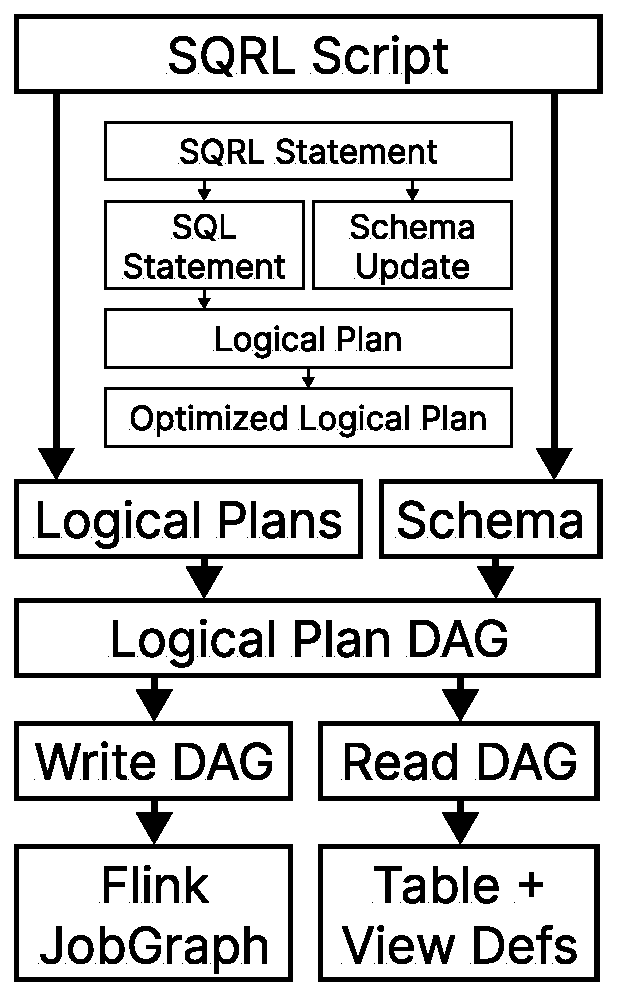
\includegraphics[width=0.7\linewidth]{compilation.pdf}
\caption{Diagram of SQRL compilation process}
\label{fig:datasqrl_compilation}
\end{figure}

The DataSQRL script compilation process is visualized in Figure~\ref{fig:datasqrl_compilation} and executes in 4 steps.

\subsubsection{Script Parsing}

The first step parses the SQRL script and compiles a script schema that contains all the tables and views defined in the script with associated logical plans.

A logical plan is an intermediate representation of an SQL query that is easier to analyze and optimize then the abstract syntax tree that is parsed out of an SQL statement. Logical plans represents a query statement in a way that is better for machine handling whereas SQL is better for human readability. A logical plan consists of a set of operator nodes that are connected into a tree or graph. Figure~\ref{fig:local_lp} shows an example of a logical plan tree as discussed below.

The SQRL compiler first parses all import statements to register the source tables that are referenced in subsequent column and view definitions. Import statements are resolved against the referenced data source to identify the source table. The schema of the source table is either extracted from a user provided schema file as an argument to the compiler or produced from the collected statistics of the source table. If the user provided schema is incompatible with the gathered statistics, an error is produced. The resulting table and schema are added to the script schema. The logical plan for the source table is a single table-scan node with information on how to read the associated data stream.

If the source table has a nested structure, multiple tables and their parent-child relationships are added to the script schema. The logical plans contain information on how to unnest the data into flat tables.

For example, when parsing the following import
\begin{lstlisting}[language=SQL]
IMPORT iotapp.MonitorGroup;
\end{lstlisting}
the compiler looks up the $MonitorGroup$ source table in the connected $iotapp$ data source. The schema for this nested table is created from the gathered statistics. The compiler then registers the $MonitorGroup$ and $MonitorGroup.machines$ tables in the script schema with an associated scan node against the source table for the logical plan.

View and columns definitions are transpiled into regular SQL. The abstract syntax tree (AST)\footnote{An abstract syntax tree is a parsed representation of an SQL query that converts the query string into a token tree so that the statement can be analyzed.} for the definition statement or expression is converted to an intermediate representation that makes it easy to replace relationships by their join definitions, expand relationship paths in expressions to sub-queries, convert nested query statements, make accommodations for primary key determination, propagate timestamps, and convert all other convenience features of SQRL to SQL. The intermediate representation then gets converted to an SQL AST which is analyzed and planned by Calcite~\cite{} to produce a logical plan and schema for the view. The schema and logical plan are added to the script schema.

For example, the transpilation process converts the $Sensors.readings$ nested view definition to the following SQL equivalent:

\begin{lstlisting}[language=SQL]
CREATE VIEW Sensors.readings AS
SELECT s.sensorid as sensorid,
       minute(r.time) as time_min,
       median(r.temperature) as temp
FROM Sensors s
     TEMPORAL JOIN SensorReading r
WHERE s.sensorid = r.sensorid
GROUP BY sensorid, time_min
\end{lstlisting}

The SQL AST for this statement is passed to Calcite for analysis to extract the schema of the resulting view (i.e. the three columns $sensorid$, $time_min$, and $temp$ with associated data types int, dateTime, and float) which is added to the script schema. The Calcite planner then produces a logical plan for this SQL statement as shown in Figure~\ref{fig:local_lp}.

\begin{figure}[h]
\centering
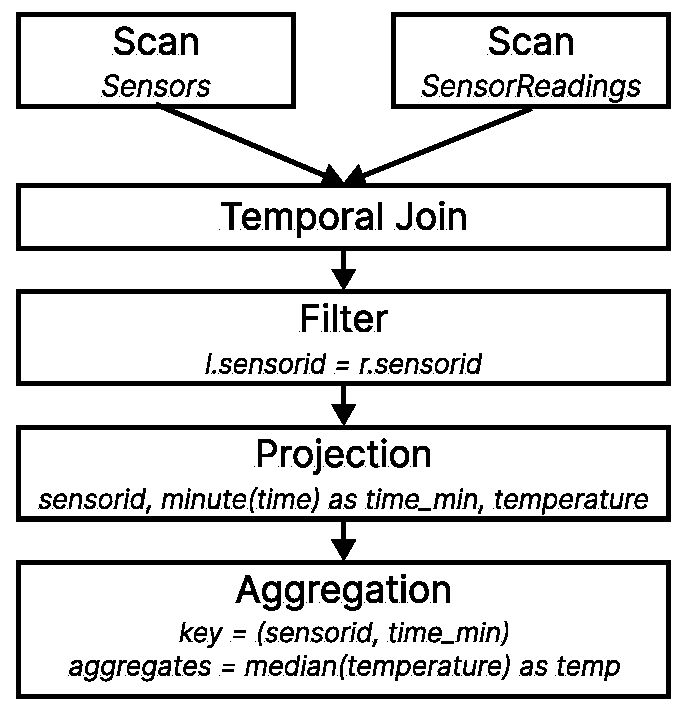
\includegraphics[width=0.7\linewidth]{local_lp.pdf}
\caption{Logical Plan for statement}
\label{fig:local_lp}
\end{figure}

The logical plan consists of scan, filter, projection, join, aggregate, window, sort, and union/except/intersect operators which are the basic operators of relational algebra. The tree structure of the logical plan prescribes the order in which the operators are applied to the input tuples.

DataSQRL uses a special join type for temporal joins which is not converted to standard SQL for efficiency reasons.

SQL does not support subscriptions natively. DataSQRL adds a dedicated "subscription" operator to the logical plan to indicate when to produce a stream from the changes against the observed view. The observed view is transpiled and converted into a logical plan as outlined above and the subscription operator is added as the new root to that logical plan tree.

The compiler converts relationships to their join definition when a relationship is used in a view definition's $FROM$ clause or expression.
When a relationship is first defined, the compiler analyzes the relationship to check validity, converts it to an intermediate representation, and registers that relationship in the script schema so it can be resolved in subsequent references.

DataSQRL uses Calcite to analyze relationship definition by converted the definition to a SQL with select-all and the table on which the relationship is defined, called the \emph{start table}, in the $FROM$ clause. For example, the $Machines.sensors$ relationship is converted to the following query for analysis:
\begin{lstlisting}[language=SQL]
SELECT * FROM Machines _
JOIN Sensors s ON
s.machineid = @.machineid
\end{lstlisting}
DataSQRL traverses the AST for this query to extract the \emph{end table} of the relationship (i.e. $Sensors$) and convert the join path and condition into an intermediate representation that can be instantiated in a view definition where the relationship is used.

For example, the relationship path $@.sensors.readings$ in the $FROM$ clause of the $Machines.hourReading$ view definition gets expanded by instantiating the two relationships to:
\begin{lstlisting}[language=SQL]
FROM Machines m JOIN Sensors s
ON s.machineid = m.machineid
JOIN Sensors.readings r
ON r.sensorid = s.sensorid
\end{lstlisting}

Appendix~\ref{appendix:sqrl2sql} describes the transpilation steps to convert an SQRL statement to a semantically equivalent SQL statement in more detail and specifically the instantiation of relationships.

For export statements, the compiler adds a mapping to the script schema that keeps track of which subscription nodes in the logical plans are exported to the given data sink.

At the end of the first step, the compiler has produced a schema and logical plan for all tables and views defined in the script.

\subsubsection{DAG Construction}

\begin{figure*}[t]
\centering
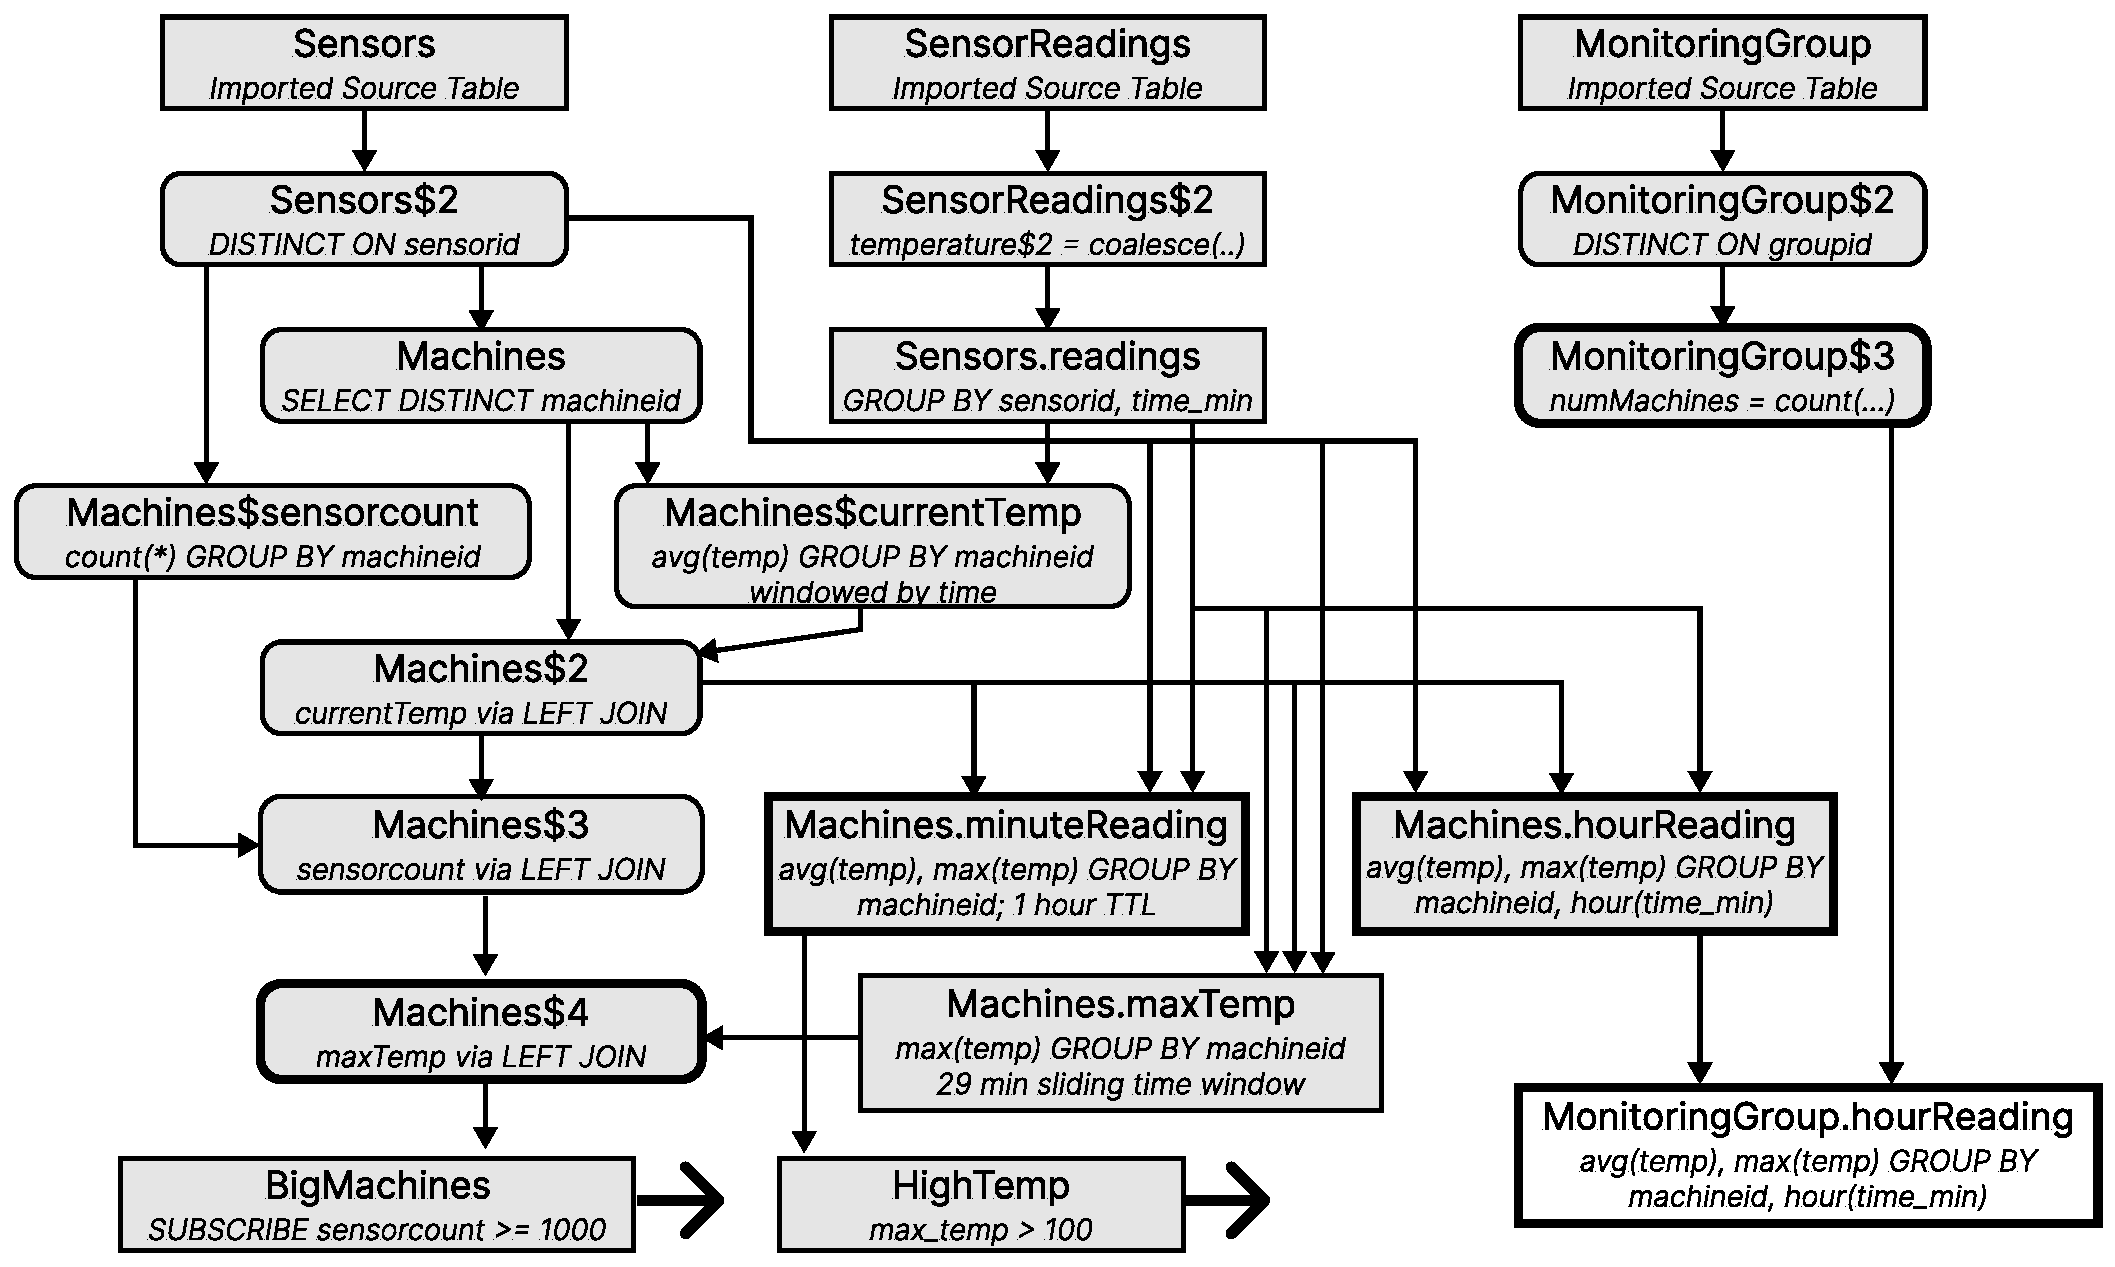
\includegraphics[width=1.0\textwidth]{logical_dag.pdf}
\caption{Logical Plan DAG for IoT Example}
\label{fig:lp_dag}
\end{figure*}

In the second step, those logical plan trees are stitched together into one logical plan directed-acyclic graph (DAG) by resolving table references of logical plan tree leafs against the schema. Specifically, for each scan node at the leaf of a logical plan tree, the compiler looks up the table that is being scanned in the schema and replaces the leaf node with the root of the logical plan tree for that table. Essentially, this process stacks logical plan trees on top of each other. The result is a DAG and not a tree because a single table can be referenced by multiple scan leaf nodes.

The result is one big connected logical plan that defines how to transform the source tables to produce all the views defined in the script. Each table in the script schema points to a node in the logical plan DAG that represents the computed table.

Figure~\ref{fig:lp_dag} shows the logical plan DAG for our IoT example. Instead of showing the full logical plan DAG, the figure shows one node per logical plan tree in order to keep the result readable. Each node in this DAG visualization includes a short description underneath the name to describe the logical plan tree that the node represents. For instance, the $Sensors.readings$ node in Figure~\ref{fig:lp_dag} represents the entire logical plan tree shown in Figure~\ref{fig:local_lp} with scan nodes for $Sensors$ and $SensorReadings$ replaced by the nodes $Sensors\$2$ and $SensorReadings\$2$ in the DAG, respectively.

During the initial script parsing, the compiler keeps track of views and columns that are redefined and overwritten in the script. We call those views and columns \emph{shadowed} and the compiler makes sure that references to such tables and columns are resolved correctly. The shadowing columns and views get an incrementing name suffix to keep the name lineage while guaranteeing unique names.

In our example, we redefine $Sensors$ as a $DISTINCT ON$ view. This new view definition now shadows the original $Sensors$ source table that was imported. That original table is now shadowed. This means that any future references to $Sensors$ resolve to the redefined view and not the original source table which is no longer referenceable but is still part of the logical plan DAG. In the logical plan DAG shown in Figure~\ref{fig:lp_dag} the shadowing $Sensors$ view is named $Sensors\$2$ and the compiler makes sure that any subsequent references to $Sensors$ in the script resolve to $Sensors\$2$ in the DAG.
Likewise, the redefined $temperature$ column on $SensorReadings$ is a shadowing column and called $temperature\$2$ in the logical plan.

All stream nodes in the DAG that are exported to an external data sink are marked with the data sink. In our example logical plan DAG in Figure~\ref{fig:lp_dag} this is indicated by a bold, horizontal arrow.

After the logical plan DAG has been assembled, the compiler analyzes the API schema definition and attaches projections for all tables/views that are exposed in the API. As described in Section~\ref{sec:sqrl_api}, each type that is exposed in the API maps onto a table or view defined in the SQRL script. Those in turn map onto nodes in the logical plan DAG. We call those nodes the \emph{API nodes} since the result sets of those nodes can be queried through the API. Projections are attached to all API nodes based on the fields that are visible in the API for the respective table or view.

The API nodes for our IoT example are highlighted by a thick border in the logical plan DAG in Figure~\ref{fig:lp_dag} based on the GraphQL API schema in Figure~\ref{fig:complete_api}. To each of those nodes we attach a projection selecting all the fields that are visible in the API. In particular, note that the $Machines$ type in the API in Figure~\ref{fig:complete_api} does not expose the $currentTemp$ field and hence it is not part of the attached projection, which allows us to project the corresponding column out during optimization and avoid unnecessary computation.

\subsubsection{DAG Cutting}
\label{sec:dag_cut}

In step three, the connected logical plan DAG is cut into two components: the write logical plan DAG ("write DAG" for short) and the read logical plan DAG (or "read DAG"). The write logical plan is the part of the logical plan DAG that gets computed incrementally as data is ingested and the results are materialized into the database or exported to downstream consumers through connected data sinks. The read logical plan DAG defines how to compute the table and view definitions exposed by the SQRL script from the materialized tables at query time in the database.
Hence, the source nodes of the read logical plan DAG are a subset of the sink nodes of the write logical plan DAG. We call those overlapping nodes the \emph{cut nodes}. The cut nodes form a cut of the original logical plan DAG and split the DAG into write and read DAGs. When cutting the DAG, the cut nodes get duplicated and are the only nodes that exist in both the write and the read DAG.

Cutting the DAG is a crucial step in the compilation of an SQRL script as it determines how much of the data computation happens at write time, i.e. as data gets ingested, versus at read time which has significant implications for the overall performance and efficiency of the resulting data service.

We discuss how to find the optimal cut in the DAG in Section~\ref{sec:dag_cut_opt}. Once the optimal cut has been determined, each node in the logical plan DAG is either labeled as "write" or as "read" depending on which side of the cut they get assigned to.

In Figure~\ref{fig:lp_dag} the write logical plan nodes are shaded in grey while the read node is white. This means that the majority of data computation for our IoT example happens at write time when data is ingested and only the $MonitoringGroup.hourReading$ view is computed at read time when answering an API request. Section~\ref{sec:dag_cut_opt} explains the rationale for this cut and the discusses the trade-offs involved.

The cut nodes in the logical plan DAG are those write nodes that are connected to read nodes. The result set for those nodes needs to be written to the database as it is incrementally computed on data ingest so that the database can compute the result sets for the read nodes on demand at query time.

In our example, $MonitoringGroup\$3$ and $Machines.hourReading$ are cut nodes since those are the only nodes connected to the single read node. The records for those two incrementally computed views get written to the database so that we can compute the $MonitoringGroup.hourReading$ view at query time by joining them.

Together, the set of cut nodes and the set of API nodes in the write DAG form the set of \emph{materialized nodes}. The incrementally computed records for the materialized nodes in the write DAG get written to the database. In our example, the materialized nodes are $Machines\$4$, $Machines.minuteReading$, $Machines.hourReading$, and $MonitoringGroup\$3$.
In addition, we call all nodes that are marked for export to data sink \emph{export nodes}. In our example, the export nodes are $BigMachines$ and $HighTemp$.

\subsubsection{Physical Plan Generation}

In step four, the write and read logical plan DAGs are converted to physical execution plans for the Flink stream engine and the database. The physical plan is a sequence of specific instructions that a computer can execute whereas a logical plan is a graph of abstract operators. To produce a physical plan, the logical operators are mapped onto physical instructions with the help of an optimizer that takes characteristics of the execution engine and the data into account. For example, a scan operator followed by a filter would be mapped onto an index lookup instructions by a database engine if the scanned table has an index for the predicate of the filter.

In other words, the logical plan is a representation of what to compute whereas a physical plan is a representation of how to execute that computation.

The write DAG is mapped onto a logical data stream in Flink using Flink's table abstraction layer which Flink optimizes to a physical execution plan in the form of a Flink JobGraph. Mapping the write DAG to a Flink data stream is mostly a direct mapping since Flink supports all the logical operators in the DAG, including temporal joins and subscriptions.

However, special consideration has to be given to filters that include the $now()$ function. $now()$ is used to express recency constraints and support computations that are based on recency. Semantically, $now()$ refers to query time, i.e. the point in time on the timeline when the API request is processed, and not the system time when data is pre-computed during the write stage. That means, we cannot evaluate $now()$ during the execution of the Flink JobGraph\footnote{Which is why the optimizer will attempt push $now()$ filters up and label them as "read" during the DAG cutting as discussed in Section~\ref{sec:dag_cut_opt}}.

Instead, we preserve the semantics of $now()$ by converting it into a sliding window or a in the Flink data stream with a window width that is equal to the time interval in the filter predicate that references $now()$ sliding interval that has $2\%$ of the length the time window.

For example, the $Machines.maxTemp$ view has the following $WHERE$ predicate referencing $now()$:
\begin{lstlisting}[language=SQL]
time_min + 24 HOUR >= now()
\end{lstlisting}
This predicate constraints the sensor readings that are aggregated in this view to be from the last 24 hours. We can rewrite this predicate to the following time interval expression:
\begin{equation}
time\_min \in [now() - 24h, now()]
\end{equation}
This gives us a 24 hour time window that advances with time, i.e. a sliding time window. By default, we advance the window every $28.8$ minutes which is two percent of 24 hours. This means we aggregate the maximum sensor temperatures for each machine in 50 time windows of 24 hours that are offset by $28.8$ minutes from each other. A sliding time window provides a good approximation for computing aggregates over recent time windows that balances memory requirements with data staleness.



Converting $now()$ predicates to sliding time windows is only supported for stream tables where the predicate constraints the timestamp of the table. Any other type of $now()$ predicate cannot be part of the write DAG.

Database sink nodes are attached to all materialization nodes in the write DAG, which inserts or upserts the incrementally computed records to the database. Similarly, all export nodes get an attached sink node that produces the records into the associated data sink.

The read DAG is converted to SQL table and view definition that are installed in the database. The cut nodes in the read DAG are converted into $CREATE TABLE$ statements to define the tables that the Flink database sink nodes insert records into. The rest of the read DAG gets incrementally converted to SQL view definitions from source to sink nodes. Those tables and views are queried by the API by mapping the script tables and views onto the physical table and view definitions through the script schema. When queried, the database produces a physical plan from the view definitions that is executed by the database to retrieve and compute the results.

All of the logical plan operators in the read DAG map to they corresponding SQL operators aside from temporal joins. Temporal joins are converted to partitioned window queries over the change stream of the state table.

Nested tables are written into a separate table in the database. If the source table has a nested structure, DataSQRL will unnest the child table, prepend the parent primary key and write the record to a separate table. For example, the $MonitoringGroup\$3$ view has a nested $machines$ table which means that records from that view get unnested and a new record is produced for each entry in $machines$ which is written to the $MonitoringGroup_machines$ table in the database.

\subsection{Optimization}
\label{sec:optimization}

The goal of the DataSQRL optimizer is to produce the most efficient implementation of the data service defined by an SQRL script and associated API schema while guaranteeing low latency response times in the API.

The DataSQRL optimizer runs during the compilation to solve the following three optimization problems:
\begin{enumerate}
    \item What is the optimal cut of the logical plan DAG?
    \item How can we identify and merge identical subgraphs in the write DAG to avoid repeat computations?
    \item What is the optimal set of indexes to install on the tables in the database?
\end{enumerate}

Each of these optimization problems is discussed in a subsection below.

All these optimization problems are solved at compile time to improve performance and efficiency at runtime. Since SQRL scripts get compiled during the deployment process of the data service has more time to find optimal solutions than a typical database query optimizer that runs at query time.

It should be noted that this section only provides detailed information on the optimization problems that are unique to DataSQRL. In addition, DataSQRL relies on the Calcite, Flink, and Postgres optimizers.

After transpiling an SQRL view definition to normal SQL and running Calcite's planner to produce a local logical plan tree as described in Section~\ref{sec:compilation}, DataSQRL runs Calcite Volcano optimizer to optimize the local logical plan. The Volcano optimizer~\cite{volcano, cascade} is a common database optimizer framework that uses a rule set for transforming logical plans in combination with a cost model to find the least costly plan through dynamic programming. DataSQRL uses Calcite's optimizer to produce locally optimal plans before combining those into the logical plan DAG in order to determine the optimal join order and push down predicates. DataSQRL provides its own cost model based on the statistics gathered during data monitoring.

In the generation of Flink's job graph, DataSQRL relies on Flink's optimizer convert the logical data stream produced from the write DAG to an optimal execution plan. Similarly, DataSQRL relies on Postgres' optimizer to convert the SQL queries issued by the DataSQRL API server to optimal execution plans against the tables in the database.

\subsubsection{Optimal DAG Cut}
\label{sec:dag_cut_opt}

Once all combinable sub-graphs have been merged, the third optimization process identifies the optimal cut of the DAG. The cut determines how much of the logical plan DAG gets incrementally maintained as data is ingested (i.e. the stream LP) and how much is computed at query time in the database (i.e. the query LP). Hence, the cut has profound implications on the overall performance of the system. The more of the logical plan DAG that gets pre-computed, the less computation the database has to perform and the faster the response times of the API. However, some joins and aggregations may be too expensive to pre-compute because of combinatorial explosion and are better computed at query time in the database when they are actually needed. Pre-computing everything is often infeasible and undesirable because of the resources it would take to do so and the time it would take to complete those computations.

To identify the optimal cut of the logical plan DAG that balances the tradeoff between pre-computation to reduce API response times and query time computation to reduce the cost and delay of pre-computation, DataSQRL employs a simple algorithm.
%Relate to graph coloring with (write/read) with the constraint that we cannot have a read node on any path between a source and a write node and we cannot have a write node on any path between a read node and a sink.
The algorithm operates in two passes over the DAG and colors the nodes in the DAG as either "write" or "read".
\begin{enumerate}
    \item Traversing the DAG from source to sink, we use a cost-based cutoff heuristic to determine if a node is labeled write or read. If the cost assigned to a node exceeds a threshold, it is marked as read, otherwise write. The algorithm stops traversing the DAG once it labeled a node as read. If the algorithm runs out of nodes to process, it labels all remaining nodes as read.
    \item For any pair of sink nodes labeled as write that share a single ancestral node N in the DAG by unique paths that only contain filter, projection, and window nodes such that the combined (generalized) filter has similar selectivity to the sum of the individual ones, combine the projections into node N' attached as a child to N and labeled write, add column-selection projections for each path and attach the paths to those projections with all those nodes marked as read. This step eliminates similar materialized tables when the cut moves all the way to the sinks.
\end{enumerate}

 We use a write-focused cost function that aims to pre-compute as much of the DAG as reasonably possible. It becomes unreasonable to pre-compute if the state we need to maintain in memory to compute an operator grows too large. Hence, our cost function assigns a cost of 0 to scan, projections and filters. Otherwise, the cost is as follows:
 \begin{enumerate}
     \item Aggregations: number of unique group by keys multiplied by the cost of each aggregate (the cost of the aggregate is the number of bytes needed to incrementally compute the aggregate divided by 8, i.e. cost(sum) = 1, cost(avg) = 2)
     \item Windows: number of unique partitions multiplied by average window width.
     \item $now()$: infinity cost if the column that is constraint by a $now()$ predicate is not the timestamp.
     \item Joins:
     \begin{enumerate}
         \item Temporal Join: Cardinality of the state table in the join
         \item If at least one table is inferred to be static: Min of the cardinalities of the static tables
         \item Stream table join with range condition on timestamps of both tables: Cardinality of records in time window. E.g. for $T1.timestamp >= T2.timestamp$ the cost is the cardinality of T2, for $T1.timestamp > T2.timestamp - 1 HOUR AND T1.timetamp < T2.timestamp + 1 HOUR$ the cost is the cardinality of 2 hours of records for T2.
         \item Other: Sum of cardinalities of both tables.
     \item Union, Intersect, Minus: Sum of cardinalities of both tables
     \end{enumerate}
 \end{enumerate}

Once the algorithm completes, all nodes are either labeled as read or write. The algorithm guarantees that this labeling produces a proper cut in the DAG, namely that we cannot have a read node on any path between a source and a write node and we cannot have a write node on any path between a read node and a sink.

%---
Talk about Machines.minuteReading and now the now() is actually part of the read DAG and gets converted to a TTL for timestamp columns.

\subsubsection{DAG Subgraph Merging}

Once the logical plan DAG has been cut, the write DAG is passed to Flink for planning and execution. However, the write DAG might contain identical subgraphs of logical plan fragments which means that the physical plan for such a DAG would compute the same results multiple times which is wasteful.

For example, in the write DAG shown in Figure~\ref{fig:lp_dag} (i.e. the gray nodes) the logical plan fragments for $Machiens.minuteReading$, $Machines.hourReading$, and $Machines.maxTemp$ all have the same three-way join between $Machines\$2$, $Sensors\$2$, and $Sensors.readings$. Incrementally computing this join on data ingest is expensive and doing it three times is very wasteful. It is more efficient to compute the join once and use the result to incrementally update all three views.

For this purpose, the DataSQRL optimizer identifies combinable sub-graphs which are merged to reduce the amount of computation. Two sub-graphs are combinable if they have the same source nodes and can be made identical by moving logical operators in a way that preserves equivalence. Unlike standard query optimization which typically pushes projections and predicates down toward the leaf nodes to reduce the size of intermediate result sets, combinable sub-graph identification requires pulling up projections, aggregations, and predicates to expose common sub-structures (e.g. joins and group-bys), merging those sub-stuctures in the DAG, and then combing the projections, aggregations, and predicates to push down the covering set.

\subsubsection{Index Selection}

The read DAG is converted to SQL table definitions for the cut nodes and SQL view definitions for any other nodes that are queried by the API. When the DataSQRL server issues a query against one of the views defined in the database, the database determines the optimal query plan to execute the query against the cut node tables which are populated by the Flink stream. The efficiency and latency of those query plans depends on the availability of suitable indexes.

For example, the API schema for our IoT data service supports requests that look up machines by $machineid$. That means, accessing the query endpoint $machines(machineid: 4)$ in the API results in the SQL query:
\begin{lstlisting}[language=SQL]
SELECT * FROM Machines$4
WHERE machineid = 4
\end{lstlisting}

Without an index on the $machineid$ column for table $Machine\$4$ this query would result in a very costly table scan that iterates through all rows to find the row with $machineid = 4$.

As discussed in Section~\ref{sec:sqrl_api}, accessing a query field or relationship field that's defined in the API schema results in a query against the table that the data type of that field maps to. The arguments provided to the field create the $WHERE$ and $ORDER BY$ clauses of that query. For relationship fields, the primary key of the table is also added as a $WHERE$ condition.

For each query and relationship field in the API schema, we generate all possible queries by combing the arguments and all possible orders into query templates. A query template is a query where the conditions have placeholder values for the arguments, like a prepared query.

For example, the $group$ query endpoint is converted to the following SQL query template using '?' as an argument placeholder:
\begin{lstlisting}[language=SQL]
SELECT * FROM MonitoringGroup$3
WHERE groupid = ?
\end{lstlisting}

The $findMachines$ query endpoint is converted to:
\begin{lstlisting}[language=SQL]
SELECT * FROM Machines$4
WHERE maxTemp > ? AND maxTemp >= ?
   AND sensorcount = ?
\end{lstlisting}

The relationship $Machines.hourReading$ supports before and after time comparison on the $time\_hour$ timestamp via the $TimeComparison$ type and is converted to:
\begin{lstlisting}[language=SQL]
SELECT * FROM Machines_hourReading
WHERE time_hour > ? AND time_hour < ?
   AND _ppk_machineid = ?
LIMIT ?
\end{lstlisting}

Here, the hidden column \emph{\_ppk\_machineid}\footnote{"ppk" stands for \emph{parent primary key}} is the primary key for the parent $Machines$ table which is automatically added to the primary key for nested tables.

The $machine$ and $machinesBySensor$ query as well as the $Machines.minuteReading$, $MonitoringGroup.machines$, and $MonitoringGroup.hourReading$ relationships are converted similarly.

All query templates are planned by Calcite into logical plans which are optimized. During optimization the filters are pushed down to the source nodes in the read DAG (i.e. the cut nodes). Those nodes represent the tables that are created in the database. For each table, all the filters that are pushed down to the corresponding source node in the DAG across all query templates are extracted and converted to conjunctive normal form (CNF). CNF is a normalized form for filter expressions where all top-level conditions are AND'ed together which makes it easier to analyze.

For example, we have 3 queries which push down filters to the $Machines\$4$ table: $machine$, $machinesBySensor$, and $findMachines$. Those filter conditions are (in order):
\begin{lstlisting}[language=SQL]
1) machineid = ?
2) sensorcount = ?
3) maxTemp > ? AND maxTemp >= ?
   AND sensorcount = ?
\end{lstlisting}

The conditions are already in CNF.

Each condition is represented as a set such that each top-level predicate constraining a column is converted to an element that captures the column name and type of constraint (i.e. equality or range). The three filter conditions for the $Machines\$4$ table are represented by the following sets:
\begin{lstlisting}[language=SQL]
1) {=machineid}
2) {=sensorcount}
3) {<>maxTemp, =sensorcount}
\end{lstlisting}

We use the symbol $<>$ to mark a range condition and $=$ to mark an equality condition. Note, multiple range conditions on the same column result in the same set element as in the case of $maxTemp$.

The sets representing filter conditions are called \emph{predicate sets}. Each set is replaced by all possible subsets based on whether the corresponding arguments are required in the API schema to match the combination of arguments that the caller of the API may provide. The first two queries only have a single required argument so the predicate sets remain the same. However, for the third query both arguments are optional which means the predicate set is replaced by its powerset\footnote{The power set of a set $S$ is the set of all subsets of $S$}:
\begin{lstlisting}[language=SQL]
1) {=machineid}
2) {=sensorcount}
3) {}, {<>maxTemp}, {=sensorcount},
   {<>maxTemp, =sensorcount}
\end{lstlisting}

The predicate sets are now combined and empty sets removed. Each predicate set is then ordered by the selectivity of the predicate condition each element represents.


 Predicate sets are ordered and pruned. The elements in a predicate set are ordered by selectivity of the predicate they represent.

We compile those query templates into logical plans and replace the table node in the logical plan by the corresponding node in the query logical plan DAG. We then optimize that combined logical plan to identify the optimal set of indexes by analyzing the filters that are pushed down to the source tables of the DAG.

\subsubsection{Hints}

Developers can add annotations to the column and view definitions in their SQRL scripts in order to provide hints to the compiler and optimizer which are used to guide the compilation and act as constraints during optimization. Hints are added before a column or view definition to which they apply.

DataSQRL supports the following annotation hints:

\begin{tabular}{|p{0.15\columnwidth}p{0.75\columnwidth}|}
 \hline
 Annotation & Description \\
 \hline
write & Enforces that the root of the logical plan for this definition is marked as "write" for DAG cutting \\
read & Enforces that the root of the logical plan for this definition is marked as "read" for DAG cutting \\
window & Overrides the defaults for time windows like the advancement time for sliding windows \\
 \hline
\end{tabular}


\section{Experiments}
\label{sec:experiments}


\section{Related Work}
\label{sec:related}

Streaming integration:

General: The SQRL query language is inspired by the work of Widom et al. on the CQL query language~\cite{arasu_cql_2006} for streaming database systems~\cite{arasu_stream_2016}.

Subscribe = Stream: Julian Hyde. 2010. Data in Flight. Commun. ACM 53, 1 (Jan. 2010), 48–52

Temporal JOIN: from Apache Flink

Unnesting Arbitrary Queries by Thomas Neumann and Alfons Kemper

Apache Calcite: A Foundational Framework for Optimized Query Processing Over Heterogeneous Data Sources

Hasura for automatic API generation

Why don't we use explicit tumble, sliding windows? Those are implementation concerns and put the burden to figure out how to optimize their program on the developer.

\section{Future Work}

better optimizers: use API statistics

snapshot isolation:
Need to propagate watermarks for each materialized table into Postgres and store them there (per partition) so that we can a) provide snapshot isolation by limiting to the max watermark across all tables involved in a query and b) determine which time buckets are closed for time buckets on stream tables that get created as views.

\section{Conclusion}
\label{sec:conclusion}



\appendix

\section{Translating SQRL to SQL}
\label{appendix:sqrl2sql}

- Every stream table has a timestamp column, denoted timestamp(table)
- A temporal join between tableA and tableB where tableA must be a stream table, i.e. "tableA TEMPORAL JOIN tableB ON ()" is equivalent to an inner join where the join condition is extended by the predicate:
    timestamp(tableA) >= timestamp(tableB)
    - if tableB is a state table:
    - if tableB is an stream table: adding condition timestamp(tableB) <= timestamp(tableA)

How we assign timestamps to streams:
    - infer: order of DISTINCT ON, column used in now() comparison, column used in time windows
        - must be of DateTime type
    - if none of the above: use \_source\_time or \_ingest\_time if former is null
    - user can define explicitly in IMPORT: IMPORT dataset.table TIMESTAMP expression
        - expression must evaluate to DateTime type
How do we get watermarks?
How can we provide snapshot isolation?

Explain now() and translation to sliding and overlapping time windows (configurable via hints)
Explain temporal joins which are assumed by default between stream and stateful or stream tables.
    - between stream and state (via DISTINCT ON): join state at time of stream event (as determined by stream timestamp)


\begin{lstlisting}[language=SQL]

#### IMPORT/EXPORT Statements

Import: Registers table in schema with columns (those tables are root nodes in the logical plan DAG)

Export: Registers an export against a defined subscription table in the schema

#### Relationship Definitions

Table.relationship := JOIN Table[1] a[1] ON condition[1]

- relationship column added to Table in schema

#### Definition Statements

### Step 1: Normalize local statements

# Normalize expression to statement
Table.column := expression
- replace expression by statement:
    SELECT expression FROM @

# Normalize local statement
Table.columnOrNested := local statement
- in validation _ resolves to Table
- if statement has single anonymous SELECT expression
    then column definition: add column to Table in schema
    else nested table definition: add nested table (with reference to Table) to schema with parent and child relationship columns and PK = Table PK + local PK for nested table (see below)
- if _ not in FROM table list (_ cannot be used as an explicit alias)
    then add "Table _" to beginning of FROM list

### Step 2: Convert local statements to global statements

# Convert local column definition to view definition
Table.column := local statement
- if statement only has _ in FROM table list and no where/group-by clause
    then: Table:= SELECT @.*, (SELECT expression from statement) AS column[+] FROM Table _
    else:
        Let statement* = statement with added WHERE clause: AND (for all PK columns pk of Table: @.pk = __.pk)
        Table:= AS SELECT __.*, (statement*) AS column[+] FROM Table __

# Convert local nested table statement to global statement
Table.nested := local statement
- Let statement* = statement with
    - add parent Table PK to select and group by:
        for all PK columns pk of Table, i=i+1: add "@.pk AS _ppk[i]" to SELECT and "@.pk" to GROUP BY
- Table.nested := statement*

### Step 3: Inline Relationships in global statements

# Convert relationships in expressions
Case 1: agg_fct(TableOrAlias.rel[1].rel[2]...rel[n].column)
=> replace with sub-query (SELECT agg_fct(_r.column) FROM TableOrAlias.rel[1].rel[2]...rel[n] AS _r)
Case 2: TableOrAlias.rel[1].rel[2]...rel[n].column if rel[i] are all to-0/1 relationships
=> replace with sub-query (SELECT _r.column FROM TableOrAlias.rel[1].rel[2]...rel[n] AS _r)

# Convert Relationships in FROM clauses
- in FROM: join or table list


### Step 4: Normalize global statements

Table := statement
- map column names for shadowed columns
- pull outer ORDER BY and LIMIT expressions as columns in SELECT and extract as meta data for Table in schema



#### Special Handling

Formally, a temporal join between a stream table $A$ and a state table $B$ is defined as:
\begin{lstlisting}[language=SQL]
A JOIN
(SELECT t.* FROM
	(SELECT s.*, row_number() OVER PARTITION BY primaryKey(B) ORDER BY s._event_time DESC AS row_no FROM (SUBSCRIBE ON CHANGE TO B) as s
	WHERE s._event_time <= timestamp(A)) as t)
WHERE t.row_no=1)

#1. DISTINCT Table ON distinct-columns ORDER BY order
- Let columns be the columns on Table
    SELECT _2.columns FROM
        (SELECT _1.*, row_number() OVER (PARTITION BY distinct-columns ORDER BY order) AS rowno
            FROM Table) _2
    WHERE rowno = 1;
- Kept as a separate construct in logical plan to convert to FLink special handlign

#2. Subscriptions
- Observed view is converted like any other statement and added to schema and logical plans
- Subscription table (with columns) is added to schema and linked to observed view with observation type (ADD, DELETE, UPDATE)
- Subscriptions are treated as CREATE TABLE statements in SQL and only materialized in flink by producing a change-stream

#3. Time Windows

Time Window functions + sliding window interpreted differently in streaming vs query (need to add watermark filter for window functions, sliding window is not continuous in streaming)

#4. UNION, etc

UNION, UNION ALL, INTERSECT, EXCEPT is supported between two stream tables if they have the same timestamp column. The semantics of these operations are the normal SQL semantics. The special SQL columns _uid, _source_time, _ingest_time are not considered in the comparison, however, the timestamp column always is. The result is a stream with the same timestamp.

UNION, UNION ALL, INTERSECT, EXCEPT is supported between two state tables if they have the same primary key. However, the semantics is different from standard SQL: the comparison is done only on the primary key columns. For UNION, INTERSECT and EXCEPT the non-primary key values of the left hand side are used for columns with the same primary key. These operations preserve the original primary key.
UNION ALL merges states and does not do primary key comparison. This operation extends the primary key by an additional column that keeps track of which table a particular record came from and to ensure that the primary key remains unique.

UNION, UNION ALL, INTERSECT, EXCEPT are not supported between stream and state tables.


#5. Windows

Window based partitioning and aggregation in the SELECT clause is not supported by SQRL.

---------------

Local Query Rewriting rules:
- sub-queries to LEFT JOIN
- eliminate identical self-joins (i.e. self joins on table PK cols)

Global (DAG) Query Rewriting rules:
- combine incremental view definitions (e.g. for adding column definitions) that are chained together in a straight line (i.e. no other dependencies) and don't reference previously defined columns

\end{lstlisting}


We infer watermark timestamp for streaming data sources and only consider closed time buckets when watermark is used in GROUP BY. However, there may be stragglers which causes retractions - even in downstream data sinks using

but detailed description from google doc in here

\section{Mapping API schema definition to SQRL}
\label{appendix:sqrl2graphql}

\begin{verbatim}
Copy https://docs.google.com/document/d/1VjO8ZYUSkp5r8rvSGKBvhYV4M30sLoPqacjUyIkonXM/edit# in here
\end{verbatim}


\section{Scrap Space}

%------------

Streaming data services need to provide low latency response times to both newly incoming data (e.g. a new user action that updates the recommendations for this user) and to user requests (e.g. a user viewing their recommendations in a mobile app). Likewise, streaming data services need to support high throughput for incoming data (e.g. the number of user action records per second) and user requests (e.g. the number of concurrent users viewing their recommendations).

Implementing streaming data services that meet these requirements is very costly, time consuming, and error prone because of the lack of suitable data technologies and a complex developer ecosystem. Because streaming data services are difficult to implement in practice, their adoption has been relatively slow outside of a few technology companies with the talent and resources to build them successfully, despite the fact that the data-driven features and data-intensive applications they facilitate can deliver significant value to an organization.

There is no single data technology that developers can use to implement a streaming data service that meets application requirements. As a consequence, actual implementations combine multiple data technologies like batch-processing, databases, ETL tools, and data warehouse that are orchestrated through fragile data pipelines and integrated with custom scripts. Such architectures require a lot of time and effort to implement and the resulting complexity makes it hard to reason about the system as a whole which causes errors and significant operational overhead.

%----------

The second obstacle to implementing streaming data services is the complexity of the developer ecosystem and poor usability. To build a streaming data service developers need to have expertise in a fragmented set of tools and languages which do not share a conceptual model, lack interoperability, and require low-level tuning. Therefore, teams implementing streaming data services tend to be large, faced with a steep learning curve, spend a lot of time writing so called \textit{"plumbing"} code that maps data between systems or schemas, and have to hand-optimize the resulting data system.

%------------

For other aspects of streaming data services, SQL is too difficult or cumbersome to use, which causes developers to choose other languages and tools. For data extraction, pre-processing, and integration, developers prefer scripting languages like Python or ETL tools. Streaming view materialization is often implemented procedurally in imperative languages like Java or Go. Developers prefer Python or R for data analysis. Queries are executed through object-relational mappers (ORM). And some data processing may be done in the user-facing application in JavaScript, Ruby, or similar web application languages.

Such a fragmented and complex developer ecosystem reduces developer productivity and makes implementing streaming data services more costly. Since developers fill perceived gaps and shortcoming in SQL with imperative languages, they have to invest a significant amount of time into finding efficient implementations for their data transformations and optimize their code by hand. A declarative language like SQL allows developers to focus on the data transformations and letting the optimizer determine the most efficient implementation. Since the choice of data structures, execution plan, and index structures matters greatly to the performance of a streaming data service, this significantly improves developer productivity.


\printbibliography

\end{document}